\documentclass[runningheads]{llncs}
%
\usepackage[T1]{fontenc}
\usepackage{graphicx}
\usepackage{times}


\usepackage{tabularx}
\usepackage{float}

\usepackage{multicol}
\usepackage{changes}
\usepackage[bookmarks=true]{hyperref}
\usepackage{amsmath}
\usepackage{mathtools}
\usepackage{textcomp}
\usepackage{algorithmic}
\usepackage[ruled,vlined,noend,linesnumbered]{algorithm2e}
\usepackage[english]{babel}
\usepackage{amssymb}
\usepackage{graphicx}
\usepackage{xcolor}
\usepackage{enumerate}
\usepackage{framed}
\usepackage{tabularx}
\usepackage{url}
\usepackage{mathrsfs}
\usepackage[framemethod=default,innerleftmargin=5pt,innerrightmargin=5pt,skipabove=5pt,topline=false,rightline=false,bottomline=false,linewidth=2.5pt,roundcorner=5pt]{mdframed}
\usepackage{paralist}
\usepackage[table]{xcolor}
\usepackage{xcolor}

\usepackage{xcolor}
\usepackage[linesnumbered,ruled,vlined]{algorithm2e}

\usepackage{pgfplots}
\pgfplotsset{compat=1.18}

\newcommand\mycommfont[1]{\footnotesize\ttfamily\textcolor{blue}{#1}}
\SetCommentSty{mycommfont}

\usepackage{complexity}

%
\begin{document}
%
\title{Gen-MOR: Generative Modeling of Dominance-Preserving Multi-Objective Plans
}
%
\author{Anjan Roy and Syed Hasnayeen}
\institute{Missouri State University, Springfield MO}
%
\maketitle
%
\begin{abstract}
The purpose of multi-objective planning is to compare plans across several competing objectives. Pareto dominance is used to distinguish nondominated plans from dominated ones. We have introduced Gen-MOR, a generative model for learning and generating dominance-preserving multi-objective plans that are derived from the Minimal Objectives Relevant to Nondominated Plans (MORNP) setting. Each plan in the dataset is represented as an objective vector with a structural level: $P^{+}$ for nondominated plans and $P^{-}$ for dominated plans.

We have trained and evaluated three neural generative models: a plain autoencoder (AE), a variational autoencoder (VAE), and a conditional variational autoencoder (CVAE). All three models are assessed using reconstruction error, classification accuracy, F1 score, and latent-space characteristics. We have introduced a novel domain-specific metric called Dominance Validity Rate (DVR), which measures whether generated plans preserve the desired dominance structure. The results show that AE and VAE learn useful representations for reconstruction and classification, and CVAE enables class-conditioned generation. Nonetheless, dominance-valid generations remain more difficult than standard reconstruction, which tells us the need for explicit dominance-aware generative modeling. 

\keywords{Generative modeling \and Multi-objective planning \and Pareto dominance \and Autoencoder \and Variational autoencoder \and Conditional VAE \and Dominance validity}
\end{abstract}
%
\section{Introduction}

Multi-objective planning problems arise when a decision maker must evaluate candidate plans using more than one objective. In many planning domains, a single scalar score is not sufficient to describe plan quality because objectives may conflict with one another. For example, one plan may minimize travel distance while another may reduce risk, energy consumption, or time. In this setting, comparing plans requires reasoning over objective vectors rather than individual values. Pareto dominance provides a principled way to perform this comparison by identifying plans that are not strictly worse than others across the selected objectives. The set of such nondominated plans forms the Pareto front and represents the trade-off boundary among competing objectives. 

This project builds on the Minimal Objectives Relevant to Nondominated Plans (MORNP) setting, where the goal is to reason about which objectives are necessary for preserving the dominance and nondominance structure among a collection of plans. In MORNP, plans can be separated into two structurally meaningful classes. The first class, denoted by $P^{+}$, contains nondominated plans that should remain relevant under the selected objective subset. The second class, denoted by $P^{-}$, contains dominated plans that should be excluded by the dominance relation. This distinction is important because the label of a plan is not simply an independent class label; it depends on how that plan relates to other plans in the objective space.

Generating large datasets for this type of reasoning is challenging. Standard synthetic data generation can create numerical vectors that appear realistic, but it may not preserve the dominance relationships that define the problem. A generated plan may have objective values that resemble the original data distribution while still violating the intended $P^{+}$ or $P^{-}$ structure. Therefore, a generative model for this domain must be evaluated not only by reconstruction quality or classification accuracy, but also by whether the generated samples remain valid under the dominance rules of the multi-objective planning problem.

To address this issue, this project proposes Gen-MOR, a generative modeling framework for learning and generating dominance-preserving multi-objective plans. Each plan is represented as an objective vector, and each vector is associated with a binary structural label indicating whether it belongs to $P^{+}$ or $P^{-}$. The central idea is to train neural generative models that can learn useful representations of these plan vectors, reconstruct existing samples, classify their dominance labels, and generate new synthetic plans that remain consistent with the MORNP structure.

The project evaluates three neural generative architectures: a plain autoencoder (AE), a variational autoencoder (VAE), and a conditional variational autoencoder (CVAE). The AE is used to study whether a compressed latent representation can preserve enough information to reconstruct objective vectors and separate $P^{+}$ from $P^{-}$. The VAE extends this idea by learning a regularized latent distribution from which new samples can be generated. The CVAE further incorporates the dominance label as a conditioning variable, allowing the model to generate samples targeted toward either the nondominated class or the dominated class. Together, these models provide a useful progression from representation learning to probabilistic generation and finally to class-controlled generation.

A key part of this project is the evaluation of generated samples using a dominance-aware metric. Standard metrics such as mean squared reconstruction error, accuracy, and F1 score are useful for measuring how well a model reconstructs or classifies existing data. However, they do not directly measure whether newly generated plans satisfy the relational structure required by Pareto dominance. For this reason, the project uses Dominance Validity Rate (DVR), a domain-specific metric that checks whether generated $P^{+}$ samples remain nondominated and whether generated $P^{-}$ samples remain dominated under the selected objective subset. DVR is therefore used as the main structural validity measure for the Gen-MOR framework.

The main contribution of this project is the formulation and experimental study of generative modeling for MORNP-style dominance-preserving plan generation. First, the project represents multi-objective plans as learnable objective vectors with dominance-based structural labels. Second, it trains AE, VAE and CVAE models to reconstruct, classify, and generate such plans. Third, it evaluates model behavior using both standard machine learning metrics and the dominance-specific DVR metric. Finally, it analyzes robustness across multiple random seeds to determine whether dominance-valid generation is stable or sensitive to training variation.

Overall, this work demonstrates that neural generative models can learn meaningful representations of multi-objective planning data, but it also shows that dominance-preserving generation is more difficult than ordinary reconstruction or classification. A model may achieve low reconstruction error while still generating samples that violate the intended dominance structure. This observation motivates the need for future generative models that incorporate dominance constraints directly into the learning objective, rather than treating dominance validity only as a post-hoc evaluation measure.
%
\section{Related Work}

Multi-objective optimization has long studied how to compare and select solutions when several objectives must be considered simultaneously. Classical formulations describe solution quality through objective vectors and use Pareto dominance to identify solutions that represent meaningful trade-offs among conflicting objectives \cite{miettinen1999nonlinear}. Evolutionary multi-objective algorithms, such as NSGA-II, further popularized Pareto-front-based reasoning by maintaining diverse sets of nondominated solutions during optimization \cite{deb2002fast}. These foundations are important for this project because Gen-MOR also relies on the distinction between nondominated and dominated plans. However, rather than directly solving a multi-objective optimization problem, Gen-MOR studies whether neural generative models can learn and generate objective-vector plans while preserving their dominance-based structure.

Generative modeling provides the learning foundation for this work. Autoencoders learn compressed representations by mapping inputs into a latent space and reconstructing them from that representation \cite{hinton2006reducing}. Variational autoencoders extend this idea by learning a probabilistic latent space, making them suitable for sampling and generation \cite{kingma2014autoencoding}. Conditional generative models further allow generation to be guided by auxiliary information, such as class labels or desired attributes \cite{sohn2015learning}. More broadly, the generative modeling literature includes adversarial models, normalizing flows, and diffusion models, each of which provides a different way to learn and sample from complex data distributions \cite{goodfellow2014generative,papamakarios2021normalizing,ho2020denoising}. Gen-MOR uses this general family of ideas, but applies them to a structured multi-objective planning setting where validity depends on dominance relationships rather than only on visual, chemical, or statistical realism.

Recent work has increasingly connected generative modeling with multi-objective optimization. Abeer et al. proposed a multi-objective latent space optimization method for generative molecular design models \cite{abeer2024multiobjective}. Their approach uses Pareto-efficiency-based weighting during iterative retraining so that the generative model becomes more likely to produce molecules with improved multi-objective trade-offs. This work is relevant because it demonstrates that Pareto information can be used to influence a learned latent generative model. However, its goal is to improve molecular candidates with respect to multiple properties, while Gen-MOR focuses on whether generated plan vectors preserve dominance labels and structural consistency.

Latent Pareto set learning provides another closely related direction. The MLPS framework studies multi-objective molecular design by learning a mapping from preference vectors to Pareto-optimal solutions in a continuous latent space \cite{mlps2024latentparetoset}. This approach addresses the limitation of producing only a small number of Pareto candidates by attempting to learn a broader representation of the Pareto set. Gen-MOR is related to this idea because it also treats latent representation learning as useful for multi-objective reasoning. The difference is that Gen-MOR does not primarily aim to approximate the entire Pareto set. Instead, it evaluates whether generated samples remain consistent with the nondominated and dominated plan classes produced by a MORNP-style setting.

More recent generative approaches have used flow-based and diffusion-based models to guide samples toward Pareto-optimal regions. ParetoFlow introduces guided flow matching for offline multi-objective optimization \cite{yuan2025paretoflow}. It uses multi-objective predictor guidance and weight vectors to encourage generated samples to cover different regions of the Pareto front. Similarly, PROUD formulates multi-objective generation as a constrained diffusion process, where generated samples should maintain generation quality while moving toward Pareto optimality \cite{yao2024proud}. These methods show that advanced generative models can be explicitly guided by multi-objective structure. Gen-MOR differs from them in evaluation emphasis: instead of only asking whether generated samples approach the Pareto front, Gen-MOR asks whether generated samples preserve their intended dominance category as $P^{+}$ or $P^{-}$.

Pareto-aware generation has also been studied in scientific design problems such as proteins and molecules. MosPro proposes a machine-learning-guided framework for multi-objective protein sequence design, using Pareto-optimal sampling to generate sequences that balance multiple protein properties \cite{luo2025mospro}. This line of work shows that Pareto-aware generation is practically important in domains where a design must satisfy several competing scientific objectives. Antoniuk et al. further show that static generative models may fail to advance the known Pareto front unless generation is combined with active learning, external verification, and iterative retraining \cite{antoniuk2026active}. This observation is especially relevant to Gen-MOR because it reinforces the need to verify generated samples using a domain-specific structural criterion rather than relying only on ordinary learning metrics.

Taken together, existing work shows that generative models can support multi-objective search, latent-space optimization, Pareto-front approximation, and scientific design. However, most of these methods focus on generating samples that improve objective values or approximate the Pareto front. Gen-MOR addresses a complementary problem: generating multi-objective plan vectors that preserve dominance-based labels. In this project, a generated $P^{+}$ sample should remain nondominated, while a generated $P^{-}$ sample should remain dominated under the selected objective subset. This motivates the use of Dominance Validity Rate (DVR) as a structural evaluation metric alongside reconstruction error, classification accuracy, and F1 score. Therefore, Gen-MOR positions itself not as another Pareto-front optimizer, but as a dominance-preserving generative modeling framework for MORNP-style multi-objective planning data.
%
\section{Problem Formulation}
\label{sec:problem_formulation}

This section formalizes the multi-objective reasoning problem used in Gen-MOR. The formulation begins with plans represented as objective vectors, then defines dominance, nondominance, and dominated plan sets. These definitions are then used to state the MORNP objective-subset problem and the Gen-MOR learning problem. Throughout this paper, we use a maximization convention: a larger objective value is considered better. If an objective is naturally a cost, such as distance or risk, it can be transformed into a maximization score before applying the same definitions.

\subsection{Multi-Objective Plan Representation}
\label{subsec:plan_representation}

Let
\begin{equation}
    \mathcal{P} = \{p_1, p_2, \ldots, p_N\}
    \label{eq:plan_set}
\end{equation}
denote a finite set of $N$ candidate plans. Each plan is evaluated using a collection of $m$ objectives,
\begin{equation}
    \Omega = \{\omega_1, \omega_2, \ldots, \omega_m\},
    \label{eq:objective_set}
\end{equation}
where each objective measures one aspect of plan quality. For example, an objective may correspond to time efficiency, energy efficiency, safety, reward, or another planning criterion.

Each plan $p_i$ is represented by an objective vector
\begin{equation}
    \mathbf{x}_i = (o_{i1}, o_{i2}, \ldots, o_{im}) \in \mathbb{R}^{m},
    \label{eq:plan_vector}
\end{equation}
where $o_{ij}$ is the value of plan $p_i$ under objective $\omega_j$. The vector $\mathbf{x}_i$ is therefore the numerical representation of plan $p_i$ used by both the dominance-checking procedure and the generative models.

In later sections, we use $p_i$ to refer to the symbolic plan and $\mathbf{x}_i$ to refer to its objective-vector representation. When the context is clear, dominance comparisons are expressed using the plan notation $p_i$, while neural models operate directly on the vector notation $\mathbf{x}_i$.

\subsection{Objective Space}
\label{subsec:objective_space}

The objective vectors for all plans can be collected into an objective matrix
\begin{equation}
    \mathbf{X}
    =
    \begin{bmatrix}
        o_{11} & o_{12} & \cdots & o_{1m} \\
        o_{21} & o_{22} & \cdots & o_{2m} \\
        \vdots & \vdots & \ddots & \vdots \\
        o_{N1} & o_{N2} & \cdots & o_{Nm}
    \end{bmatrix}
    \in \mathbb{R}^{N \times m}.
    \label{eq:objective_matrix}
\end{equation}
Each row of $\mathbf{X}$ corresponds to one plan, and each column corresponds to one objective. The full objective space is therefore the $m$-dimensional space in which each plan is represented as a point.

In the MORNP setting, dominance may be evaluated using only a subset of objectives. Let
\begin{equation}
    S \subseteq \Omega
    \label{eq:selected_objective_subset}
\end{equation}
denote a selected objective subset. If $S$ contains $k$ objectives, then $|S|=k$. The projection of a plan vector $\mathbf{x}_i$ onto the selected objectives is denoted by
\begin{equation}
    \mathbf{x}_i^{S} = (o_{ij})_{\omega_j \in S}.
    \label{eq:selected_projection}
\end{equation}
This projected vector contains only the objective values used for dominance comparison under $S$.

\subsection{Pareto Dominance Relation}
\label{subsec:pareto_dominance}

Given a selected objective subset $S \subseteq \Omega$, plan $p_a$ Pareto dominates plan $p_b$ under $S$ if $p_a$ is at least as good as $p_b$ on every selected objective and strictly better on at least one selected objective. Under the maximization convention, this dominance relation is defined as
\begin{equation}
    p_a \succ_S p_b
    \iff
    \left(
    \forall \omega_j \in S,\; o_{aj} \geq o_{bj}
    \right)
    \land
    \left(
    \exists \omega_k \in S,\; o_{ak} > o_{bk}
    \right).
    \label{eq:pareto_dominance}
\end{equation}
Here, $\succ_S$ denotes strict Pareto dominance with respect to the selected objective subset $S$.

This definition is central to the rest of the paper. A plan's dominance status is not determined by its objective vector alone; it is determined by comparing that vector against other plan vectors. Therefore, dominance is a relational property over a set of plans.

\subsection{Nondominated Plan Set $P^{+}$}
\label{subsec:nondominated_plan_set}

A plan is nondominated under $S$ if there is no plan in the reference plan set that dominates it. Using the dominance relation from Eq.~\eqref{eq:pareto_dominance}, the nondominated plan set is defined as
\begin{equation}
    P^{+}_{S}
    =
    \left\{
    p_i \in \mathcal{P}
    \;\middle|\;
    \nexists p_j \in \mathcal{P}
    \text{ such that }
    p_j \succ_S p_i
    \right\}.
    \label{eq:p_plus_definition}
\end{equation}
The set $P^{+}_{S}$ contains the plans that remain relevant under the selected objectives because no other plan is strictly better according to the Pareto dominance relation.

In this paper, $P^{+}$ is used to denote the target nondominated class produced by the MORNP-style data construction. When the selected objective subset is clear from context, we write $P^{+}$ instead of $P^{+}_{S}$.

\subsection{Dominated Plan Set $P^{-}$}
\label{subsec:dominated_plan_set}

A plan is dominated under $S$ if at least one other plan dominates it. The dominated plan set is therefore defined as
\begin{equation}
    P^{-}_{S}
    =
    \left\{
    p_i \in \mathcal{P}
    \;\middle|\;
    \exists p_j \in \mathcal{P}
    \text{ such that }
    p_j \succ_S p_i
    \right\}.
    \label{eq:p_minus_definition}
\end{equation}
The set $P^{-}_{S}$ contains plans that are excluded by the dominance relation because another plan is at least as good on all selected objectives and strictly better on at least one selected objective.

As with $P^{+}$, we write $P^{-}$ when the selected objective subset is clear. In the Gen-MOR dataset, $P^{+}$ and $P^{-}$ are used as the two structural classes for learning. A plan in $P^{+}$ receives the positive label, while a plan in $P^{-}$ receives the negative label.

\subsection{MORNP Problem Definition}
\label{subsec:mornp_definition}

\begin{problem}[MORNP Problem]
    The Minimal Objectives Relevant to Nondominated Plans problem, abbreviated as MORNP, asks whether a small subset of objectives can preserve a desired dominance structure among plans. The motivation is that not every objective may be necessary to explain why some plans are nondominated and others are dominated. Therefore, MORNP seeks a compact objective subset that maintains the classification of plans into $P^{+}$ and $P^{-}$.
\end{problem}
\textcolor{red}{Make this definition formal. Indicate what are the inputs and the output of the problem.}



Let $P^{+}_{\text{tar}}$ denote the target set of plans that should remain nondominated, and let $P^{-}_{\text{tar}}$ denote the target set of plans that should remain dominated. A selected objective subset $S \subseteq \Omega$ is considered feasible if it satisfies both conditions:
\begin{equation}
    \forall p_i \in P^{+}_{\text{tar}},
    \quad
    \nexists p_j \in \mathcal{P}
    \text{ such that }
    p_j \succ_S p_i,
    \label{eq:mornp_positive_condition}
\end{equation}
and
\begin{equation}
    \forall p_i \in P^{-}_{\text{tar}},
    \quad
    \exists p_j \in \mathcal{P}
    \text{ such that }
    p_j \succ_S p_i.
    \label{eq:mornp_negative_condition}
\end{equation}
Eq.~\eqref{eq:mornp_positive_condition} ensures that every target positive plan remains nondominated under the selected objectives. Eq.~\eqref{eq:mornp_negative_condition} ensures that every target negative plan remains dominated under the selected objectives.

The optimization version of MORNP can then be written as
\begin{equation}
    S^{*}
    =
    \arg\min_{S \subseteq \Omega}
    |S|
    \quad
    \text{subject to}
    \quad
    S \text{ satisfies Eq.~\eqref{eq:mornp_positive_condition} and Eq.~\eqref{eq:mornp_negative_condition}}.
    \label{eq:mornp_optimization}
\end{equation}
The decision version asks whether there exists a feasible subset $S$ such that
\begin{equation}
    |S| \leq k,
    \label{eq:mornp_decision}
\end{equation}
where $k$ is a given objective budget.

This formulation provides the structural basis for Gen-MOR. The generated data consists of objective vectors whose labels are meaningful only because they satisfy the dominance and nondominance conditions induced by a selected objective subset.

\subsection{Gen-MOR Learning Problem}
\label{subsec:genmor_learning_problem}

Gen-MOR transforms the MORNP-style dominance structure into a generative learning problem. Given the objective matrix $\mathbf{X}$ from Eq.~\eqref{eq:objective_matrix}, each plan vector $\mathbf{x}_i$ is assigned a binary label
\begin{equation}
    y_i =
    \begin{cases}
        1, & \text{if } p_i \in P^{+},\\
        0, & \text{if } p_i \in P^{-}.
    \end{cases}
    \label{eq:label_definition}
\end{equation}
The resulting supervised generative dataset is
\begin{equation}
    \mathcal{D}
    =
    \{(\mathbf{x}_i, y_i)\}_{i=1}^{N}.
    \label{eq:genmor_dataset}
\end{equation}

The objective of Gen-MOR is to learn a model that captures both the numerical structure of objective vectors and the dominance-based class structure. More specifically, the learned model should support four tasks:
\begin{compactenum}
    \item reconstructing input objective vectors,
    \item classifying objective vectors as $P^{+}$ or $P^{-}$,
    \item generating new synthetic objective vectors, and
    \item preserving dominance validity in generated samples.
\end{compactenum}

Let $G_{\theta}$ denote a generative model with parameters $\theta$. Depending on the model architecture, $G_{\theta}$ may generate a new vector from a latent variable $\mathbf{z}$, or from both a latent variable and a class label. For unconditional generation, the model can be written as
\begin{equation}
    \tilde{\mathbf{x}} = G_{\theta}(\mathbf{z}),
    \quad
    \mathbf{z} \sim p(\mathbf{z}),
    \label{eq:unconditional_generation}
\end{equation}
where $\tilde{\mathbf{x}}$ is a generated objective vector. For class-conditioned generation, as in a CVAE, generation can be written as
\begin{equation}
    \tilde{\mathbf{x}} = G_{\theta}(\mathbf{z}, y),
    \quad
    \mathbf{z} \sim p(\mathbf{z}),
    \quad
    y \in \{0,1\}.
    \label{eq:conditional_generation}
\end{equation}
The conditional form is especially useful in Gen-MOR because it allows the model to generate samples intended to belong to $P^{+}$ or $P^{-}$.

A generated vector $\tilde{\mathbf{x}}$ is not considered successful merely because it is numerically plausible. It must also satisfy the dominance condition associated with its intended label. This requirement motivates the Dominance Validity Rate metric defined next.

\subsection{Dominance Validity Rate, DVR}
\label{subsec:dvr}

Dominance Validity Rate (DVR) measures whether generated samples preserve the dominance structure expected from their intended class. Let
\begin{equation}
    \tilde{\mathcal{P}}^{+}
    =
    \{\tilde{p}^{+}_1, \tilde{p}^{+}_2, \ldots, \tilde{p}^{+}_{M_{+}}\}
    \label{eq:generated_positive_set}
\end{equation}
denote generated samples intended to belong to $P^{+}$, and let
\begin{equation}
    \tilde{\mathcal{P}}^{-}
    =
    \{\tilde{p}^{-}_1, \tilde{p}^{-}_2, \ldots, \tilde{p}^{-}_{M_{-}}\}
    \label{eq:generated_negative_set}
\end{equation}
denote generated samples intended to belong to $P^{-}$. Each generated plan $\tilde{p}$ has an objective-vector representation $\tilde{\mathbf{x}}$.

For dominance verification, let
\begin{equation}
    \mathcal{V}
    =
    \mathcal{P}
    \cup
    \tilde{\mathcal{P}}^{+}
    \cup
    \tilde{\mathcal{P}}^{-}
    \label{eq:verification_pool}
\end{equation}
denote the verification pool containing the original reference plans and the generated plans. The same selected objective subset $S$ is used for all dominance checks.

\subsubsection{Positive Dominance Validity Rate}
\label{subsubsec:positive_dvr}

A generated positive sample is valid if it remains nondominated under the selected objective subset. The positive DVR is defined as
\begin{equation}
    \operatorname{DVR}^{+}
    =
    \frac{1}{M_{+}}
    \sum_{i=1}^{M_{+}}
    \mathbb{I}
    \left[
    \nexists q \in \mathcal{V}
    \text{ such that }
    q \succ_S \tilde{p}^{+}_i
    \right],
    \label{eq:positive_dvr}
\end{equation}
where $\mathbb{I}[\cdot]$ is the indicator function, returning $1$ if the condition is true and $0$ otherwise. A higher $\operatorname{DVR}^{+}$ means that more generated $P^{+}$ samples remain nondominated.

\subsubsection{Negative Dominance Validity Rate}
\label{subsubsec:negative_dvr}

A generated negative sample is valid if it is dominated by at least one other plan under the selected objective subset. The negative DVR is defined as
\begin{equation}
    \operatorname{DVR}^{-}
    =
    \frac{1}{M_{-}}
    \sum_{i=1}^{M_{-}}
    \mathbb{I}
    \left[
    \exists q \in \mathcal{V}
    \text{ such that }
    q \succ_S \tilde{p}^{-}_i
    \right].
    \label{eq:negative_dvr}
\end{equation}
A higher $\operatorname{DVR}^{-}$ means that more generated $P^{-}$ samples correctly remain dominated.

The overall DVR can be reported as a weighted average of positive and negative validity:
\begin{equation}
    \operatorname{DVR}
    =
    \frac{
        M_{+}\operatorname{DVR}^{+}
        +
        M_{-}\operatorname{DVR}^{-}
    }{
        M_{+}+M_{-}
    }.
    \label{eq:overall_dvr}
\end{equation}
When class-specific behavior is important, $\operatorname{DVR}^{+}$ and $\operatorname{DVR}^{-}$ are reported separately.

\subsubsection{Why DVR Is Needed?}
\label{subsubsec:why_dvr_needed}

Standard machine learning metrics are necessary but not sufficient for Gen-MOR. Reconstruction mean squared error measures whether a model can reproduce objective vectors. Classification accuracy and F1 score measure whether a model can separate $P^{+}$ and $P^{-}$ labels on observed data. However, none of these metrics directly checks whether newly generated samples satisfy the dominance relation in Eq.~\eqref{eq:pareto_dominance}.

This distinction is important because dominance validity is relational. A generated vector may have low reconstruction error or may be classified as $P^{+}$ by a neural classifier, but it may still be dominated by another plan when checked using the formal Pareto relation. Similarly, a generated $P^{-}$ sample may appear numerically plausible but fail to be dominated by any other plan. DVR is therefore introduced as a structural validity metric that directly evaluates whether generated samples preserve the MORNP-style dominance requirements.
%
\section{Dataset Generation and Verification}
\label{sec:dataset_generation}

This section describes how the Gen-MOR dataset is generated, labeled, verified, and exported for neural generative modeling. The dataset is constructed from the MORNP-style dominance setting defined in Section~\ref{sec:problem_formulation}. Each sample corresponds to one plan represented by an objective vector, and each plan is assigned a dominance-based label indicating whether it belongs to the nondominated class $P^{+}$ or the dominated class $P^{-}$. The final dataset used in this experiment contains $50{,}000$ plans, with $25{,}209$ plans in $P^{+}$ and $24{,}791$ plans in $P^{-}$.

\subsection{MORNP-Based Synthetic Plan Generation}
\label{subsec:mornp_based_generation}

The dataset is generated as a synthetic MORNP-style plan collection. Let $\mathcal{P}$ denote the set of generated plans, as defined in Eq.~\eqref{eq:plan_set}, and let each plan $p_i \in \mathcal{P}$ be represented by an objective vector $\mathbf{x}_i \in \mathbb{R}^{m}$, as defined in Eq.~\eqref{eq:plan_vector}. The purpose of the synthetic generator is to create plan vectors that are not only numerical samples, but also dominance-structured samples. Therefore, the generation process must produce both nondominated examples and dominated examples under the selected objective subset $S$.

In this experiment, the generator constructs objective vectors and then partitions them into two sets according to the Pareto dominance relation in Eq.~\eqref{eq:pareto_dominance}. Plans that satisfy the nondominance condition are placed in $P^{+}$, while plans that satisfy the dominated condition are placed in $P^{-}$. This construction makes the dataset suitable for the Gen-MOR learning problem defined in Eq.~\eqref{eq:genmor_dataset}, where each sample contains an objective vector and a binary dominance label.

The important point is that the labels are not arbitrary class annotations. They are derived from the formal dominance behavior of the plans under the selected objective subset. Therefore, the dataset generation step also serves as the first stage of structural validation.

\subsection{Objective Configuration}
\label{subsec:objective_configuration}

Each plan is evaluated using a fixed set of $m$ objectives. Following the notation from Eq.~\eqref{eq:objective_set}, the full objective set is
\begin{equation}
    \Omega = \{\omega_1, \omega_2, \ldots, \omega_m\}.
    \label{eq:dataset_full_objective_set}
\end{equation}
In the implementation, these objectives are represented using names such as \texttt{obj\_1}, \texttt{obj\_2}, $\ldots$, \texttt{obj\_m}. The uploaded dataset schema uses twenty total objectives, represented as \texttt{obj\_1} through \texttt{obj\_20}. Thus, for this experiment,
\begin{equation}
    m = 20.
    \label{eq:dataset_objective_count}
\end{equation}

Dominance verification is performed using a selected subset of objectives rather than necessarily using all objectives. Let
\begin{equation}
    S = \{\omega_{s_1}, \omega_{s_2}, \ldots, \omega_{s_k}\} \subseteq \Omega
    \label{eq:dataset_selected_objective_set}
\end{equation}
denote the selected objective subset, where $k = |S|$. The sample dataset file records this selected subset explicitly under the field \texttt{selected\_objectives}. In the sample export, $k=12$, and the selected objectives include entries such as \texttt{obj\_4}, \texttt{obj\_1}, \texttt{obj\_9}, and other selected objective names.

For every plan $p_i$, the full feature vector $\mathbf{x}_i$ contains all $m$ objective values, while dominance checks are computed using the projected vector $\mathbf{x}_i^{S}$ from Eq.~\eqref{eq:selected_projection}. This distinction is important because the generative models are trained on full objective vectors, but the structural validity of a generated sample is evaluated using the selected objective subset.

\subsection{Plan Construction Strategy}
\label{subsec:plan_construction_strategy}

The construction strategy is designed to produce both $P^{+}$ and $P^{-}$ samples. A naive random generator may produce a heavily imbalanced dataset because, in high-dimensional objective spaces, many randomly generated points may become nondominated. This makes it difficult to obtain enough dominated plans for learning. Therefore, the construction process explicitly controls the number of positive and negative samples.

The final experiment produces a near-balanced class distribution:
\begin{equation}
    |P^{+}| = 25{,}209,
    \qquad
    |P^{-}| = 24{,}791.
    \label{eq:balanced_dataset_counts}
\end{equation}
Thus, the total number of generated plans is
\begin{equation}
    N = |P^{+}| + |P^{-}| = 50{,}000.
    \label{eq:total_dataset_count}
\end{equation}

The construction process can be described as an iterative candidate-generation and verification procedure. Candidate plans are first generated as objective vectors. Each candidate is then tested against the selected objective subset $S$ using the dominance relation in Eq.~\eqref{eq:pareto_dominance}. If the candidate is not dominated by any relevant plan, it is eligible for the $P^{+}$ set. If it is dominated by at least one relevant plan, it is eligible for the $P^{-}$ set. The process continues until the required number of positive and negative plans is reached.

This strategy ensures that the dataset is not simply a collection of random vectors. Instead, it is a structured collection of objective vectors whose labels are justified by dominance checks. This is essential for Gen-MOR because the later generative models are expected to learn from the dominance structure and not only from the marginal distribution of objective values.

\subsection{Label Assignment}
\label{subsec:label_assignment}

After construction and verification, each plan is assigned a binary label. The label convention follows Eq.~\eqref{eq:label_definition}. A plan in the nondominated set receives label $1$, and a plan in the dominated set receives label $0$:
\begin{equation}
    y_i =
    \begin{cases}
        1, & \text{if } p_i \in P^{+},\\
        0, & \text{if } p_i \in P^{-}.
    \end{cases}
    \label{eq:dataset_label_assignment}
\end{equation}

The exported dataset also stores a text version of the class name. Plans with $y_i=1$ are stored with \texttt{set\_name} equal to \texttt{P+}, while plans with $y_i=0$ are stored with \texttt{set\_name} equal to \texttt{P-}. This redundant representation is useful during debugging because the numerical label and the symbolic class name can be checked against each other.

The learning dataset can therefore be written as
\begin{equation}
    \mathcal{D}_{\text{Gen-MOR}}
    =
    \{(\mathbf{x}_i, y_i)\}_{i=1}^{50000},
    \label{eq:final_genmor_dataset}
\end{equation}
where $\mathbf{x}_i \in \mathbb{R}^{20}$ and $y_i \in \{0,1\}$.

\subsection{Dataset Statistics}
\label{subsec:dataset_statistics}

The final dataset used in this experiment contains $50{,}000$ total plan vectors. The dataset is almost balanced between the two dominance classes. Table~\ref{tab:dataset_statistics} summarizes the class distribution.

\begin{table}[H]
\centering
\caption{Class distribution of the final Gen-MOR dataset.}
\label{tab:dataset_statistics}
\begin{tabular}{|l|c|c|c|}
\hline
\textbf{Class} & \textbf{Symbol} & \textbf{Label} & \textbf{Number of Plans} \\
\hline
Nondominated plans & $P^{+}$ & $1$ & $25{,}209$ \\
Dominated plans & $P^{-}$ & $0$ & $24{,}791$ \\
\hline
Total & -- & -- & $50{,}000$ \\
\hline
\end{tabular}
\end{table}

The class balance can also be written as
\begin{equation}
    \frac{|P^{+}|}{N} = 0.50418,
    \qquad
    \frac{|P^{-}|}{N} = 0.49582.
    \label{eq:class_balance}
\end{equation}
This balanced setup is different from the preliminary dataset used earlier in the project presentation, where the class distribution was smaller and imbalanced. In that preliminary setting, the dataset contained $829$ $P^{+}$ plans and $171$ $P^{-}$ plans. The final experiment uses a larger and balanced dataset to reduce the risk that model performance is dominated by the majority class.

\subsection{Class Imbalance}
\label{subsec:class_imbalance}

Class imbalance is a natural issue in MORNP-style data generation. In high-dimensional objective spaces, many randomly sampled plans may be nondominated because it becomes less likely that one plan is better than another across all selected objectives. As a result, a purely random construction process may produce many more $P^{+}$ samples than $P^{-}$ samples. This was observed in the earlier preliminary dataset, where the number of nondominated plans was much larger than the number of dominated plans.

Class imbalance can affect learning in several ways. A classifier trained on an imbalanced dataset may learn to favor the majority class. A generative model may also learn a latent distribution that represents $P^{+}$ more strongly than $P^{-}$, making it harder to generate dominated plans reliably. This is especially important for the CVAE because class-conditioned generation requires the model to learn both class-conditional distributions.

To reduce these issues in the final experiment, the dataset is constructed to be nearly balanced:
\begin{equation}
    |P^{+}| \approx |P^{-}|,
    \qquad
    |P^{+}| = 25{,}209,
    \qquad
    |P^{-}| = 24{,}791.
    \label{eq:balanced_class_condition}
\end{equation}
This near balance makes accuracy easier to interpret and makes F1 score, reconstruction error, and Dominance Validity Rate more comparable across the two classes.

\subsection{Dominance Verification Procedure}
\label{subsec:dominance_verification_procedure}

A sample-based verification is reported for scalability, using the Pareto dominance relation defined in Eq.~\eqref{eq:pareto_dominance}. The verification procedure uses the selected objective subset $S$ and compares each plan against the relevant plan pool.

For a candidate positive plan $p_i \in P^{+}$, the verification condition is
\begin{equation}
    \nexists p_j \in \mathcal{P}
    \text{ such that }
    p_j \succ_S p_i.
    \label{eq:positive_verification_condition}
\end{equation}
This condition is the same nondominance requirement used in Eq.~\eqref{eq:p_plus_definition}. It ensures that a positive plan is not dominated by any other plan under the selected objectives.

For a candidate negative plan $p_i \in P^{-}$, the verification condition is
\begin{equation}
    \exists p_j \in \mathcal{P}
    \text{ such that }
    p_j \succ_S p_i.
    \label{eq:negative_verification_condition}
\end{equation}
This condition is the same dominated-plan requirement used in Eq.~\eqref{eq:p_minus_definition}. It ensures that a negative plan has at least one dominator under the selected objectives.

The verification step is necessary because the dataset is later used as ground truth for training and evaluation. If the labels were not checked against the dominance relation, the neural models could learn from inconsistent examples. In the experiment, dominance verification is performed using the selected objective subset and vectorized comparison. Because a full pairwise dominance check over all $50{,}000$ plans is computationally expensive, the notebook also reports a sample-based verification over $2{,}000$ plans. This spot-check found zero $P^{+}$ dominance violations, confirming that sampled positive plans remained nondominated in the sampled reference pool. For $P^{-}$ plans, the sample-based check is more conservative because a dominated plan may require a dominator outside the sampled reference pool; therefore, negative-plan verification is interpreted with respect to the available reference set used in the check.

\subsection{Consistency Checks}
\label{subsec:consistency_checks}

Several consistency checks are applied before the dataset is accepted for training. These checks ensure that the exported records, numerical feature vectors, and dominance labels agree with each other.

First, the intended consistency condition for every $P^{+}$ plan is the nondominance condition:
\begin{equation}
    \forall p_i \in P^{+},
    \quad
    \nexists p_j \in \mathcal{P}
    \text{ such that }
    p_j \succ_S p_i.
    \label{eq:consistency_positive}
\end{equation}
%
A sample-based dominance check was performed over $2{,}000$ plans. Within this sampled reference pool, no sampled $P^{+}$ plan was found to be dominated by another sampled plan.
%
\newline
%
Second, the intended consistency condition for every $P^{-}$ plan is the dominated condition:
\begin{equation}
    \forall p_i \in P^{-},
    \quad
    \exists p_j \in \mathcal{P}
    \text{ such that }
    p_j \succ_S p_i.
    \label{eq:consistency_negative}
\end{equation}
For $P^{-}$ plans, the observed result depends on the size and coverage of the reference pool used during verification, since a negative plan may be dominated by a plan outside a sampled subset.
%
\newline
%
Third, each objective vector must have the expected dimensionality:
\begin{equation}
    \mathbf{x}_i \in \mathbb{R}^{20}
    \quad
    \forall i \in \{1,2,\ldots,N\}.
    \label{eq:feature_dimension_check}
\end{equation}
Fourth, the exported label must match the symbolic class name:
\begin{equation}
    y_i = 1 \iff \texttt{set\_name}(p_i)=\texttt{P+},
    \qquad
    y_i = 0 \iff \texttt{set\_name}(p_i)=\texttt{P-}.
    \label{eq:label_setname_consistency}
\end{equation}

Finally, the feature vector order must be consistent across all records. This is important because the neural models treat each feature position as a fixed objective dimension. If one record stores \texttt{obj\_2} in the second position but another record changes the order, then the input matrix would no longer represent a valid objective space. Therefore, every record is checked against the same \texttt{feature\_vector\_order}.

\subsection{Dataset Export Format}
\label{subsec:dataset_export_format}

The dataset is exported in JSON format so that both the metadata and the plan records are preserved. The top-level JSON object contains a dataset type, creation timestamp, metadata, an instance summary, and the list of plan records. The metadata stores the seed, full objective list, selected objective list, target plan count, constructed class counts, construction success flag, objective count, and selected objective budget $k$.

Each plan record contains the following fields:
\begin{compactitem}
    \item \texttt{plan\_name}: a unique plan identifier such as \texttt{p\_1};
    \item \texttt{label}: the binary class label, where $1$ indicates $P^{+}$ and $0$ indicates $P^{-}$;
    \item \texttt{set\_name}: the symbolic class name, either \texttt{P+} or \texttt{P-};
    \item \texttt{objective\_values}: a dictionary mapping objective names to objective values;
    \item \texttt{feature\_vector\_order}: the fixed objective order used to construct the neural input vector;
    \item \texttt{feature\_vector}: the numerical vector $\mathbf{x}_i$ used for model training.
\end{compactitem}

A simplified version of one exported record is shown below:
\begin{verbatim}
{
  "plan_name": "p_1",
  "label": 1,
  "set_name": "P+",
  "objective_values": {
    "obj_1": 48,
    "obj_2": 86,
    "...": "...",
    "obj_20": 89
  },
  "feature_vector_order": [
    "obj_1", "obj_2", "...", "obj_20"
  ],
  "feature_vector": [
    48, 86, "...", 89
  ]
}
\end{verbatim}

For training in Google Colab, the JSON records are converted into an input matrix and a label vector:
\begin{equation}
    \mathbf{X}
    =
    \begin{bmatrix}
        \mathbf{x}_1^{T} \\
        \mathbf{x}_2^{T} \\
        \vdots \\
        \mathbf{x}_N^{T}
    \end{bmatrix}
    \in \mathbb{R}^{50000 \times 20},
    \qquad
    \mathbf{y}
    =
    \begin{bmatrix}
        y_1 \\
        y_2 \\
        \vdots \\
        y_N
    \end{bmatrix}
    \in \{0,1\}^{50000}.
    \label{eq:training_matrix_and_labels}
\end{equation}
The matrix $\mathbf{X}$ is used as the numerical input to the AE, VAE, and CVAE models, while $\mathbf{y}$ is used for classification and conditional generation. The selected objective subset $S$ is retained separately because it is required for dominance verification and DVR computation after generation.
%
\section{Model Architectures}
\label{sec:model_architectures}

This section describes the neural architectures used in Gen-MOR to learn from the MORNP-based dataset defined in Section~\ref{sec:dataset_generation}. The input to every model is a plan objective vector $\mathbf{x}_i \in \mathbb{R}^{20}$ from Eq.~\eqref{eq:final_genmor_dataset}. Each vector is associated with a label $y_i \in \{0,1\}$, where $y_i=1$ indicates a nondominated plan in $P^{+}$ and $y_i=0$ indicates a dominated plan in $P^{-}$. The goal of the models is not only to reconstruct objective vectors, but also to learn a latent representation that is useful for classification and generation.

\subsection{Overview of the Gen-MOR Modeling Pipeline}
\label{subsec:modeling_pipeline}

The Gen-MOR modeling pipeline follows a common structure across the three architectures. First, the objective vector $\mathbf{x}_i$ is passed through an encoder network. The encoder maps the high-dimensional plan vector into a lower-dimensional latent representation. This latent representation is intended to capture the important structure of the plan, including information useful for distinguishing $P^{+}$ plans from $P^{-}$ plans.

For a general encoder $E_{\theta}$, the latent representation can be written as
\begin{equation}
    \mathbf{z}_i = E_{\theta}(\mathbf{x}_i),
    \label{eq:generic_encoder}
\end{equation}
where $\mathbf{z}_i \in \mathbb{R}^{d_z}$ and $d_z$ is the latent dimension. The latent vector is then passed to a decoder $D_{\phi}$ that reconstructs the original objective vector:
\begin{equation}
    \hat{\mathbf{x}}_i = D_{\phi}(\mathbf{z}_i).
    \label{eq:generic_decoder}
\end{equation}
Here, $\hat{\mathbf{x}}_i$ is the reconstructed version of $\mathbf{x}_i$.

In addition to reconstruction, the latent representation may be connected to a classifier head $C_{\psi}$ that predicts the dominance label:
\begin{equation}
    \hat{y}_i = C_{\psi}(\mathbf{z}_i),
    \label{eq:generic_classifier}
\end{equation}
where $\hat{y}_i \in [0,1]$ represents the predicted probability that plan $p_i$ belongs to $P^{+}$. This allows the model to learn a latent space that supports both reconstruction and dominance-label separation.

The three models used in this project differ mainly in how they define and use the latent representation. The plain autoencoder learns a deterministic latent vector. The variational autoencoder learns a probabilistic latent distribution from which new vectors can be sampled. The conditional variational autoencoder additionally uses the class label as a conditioning variable, which enables controlled generation of $P^{+}$ or $P^{-}$ samples.

In the implemented Gen-MOR 50K experiment, all three models use input objective vectors of dimension $20$, hidden layers of sizes $256$ and $128$, and a latent dimension of $d_z=16$. Hidden layers use batch normalization and ReLU activations, and the decoder output uses a sigmoid activation because the objective vectors are MinMax-normalized to the range $[0,1]$ before training.

%
\begin{table}[H]
\centering
\caption{Implemented neural architecture dimensions in the Gen-MOR 50K experiment.}
\label{tab:implemented_architecture}
\begin{tabular}{|l|c|c|c|}
\hline
\textbf{Component} & \textbf{AE} & \textbf{VAE} & \textbf{CVAE} \\
\hline
Input dimension & $20$ & $20$ & $21$ with label conditioning \\
Hidden dimensions & $[256,128]$ & $[256,128]$ & $[256,128]$ \\
Latent dimension & $16$ & $16$ & $16$ \\
Decoder input & $16$ & $16$ & $17$ with label conditioning \\
Decoder output & $20$ & $20$ & $20$ \\
Classifier head & $16 \rightarrow 32 \rightarrow 1$ & $16 \rightarrow 32 \rightarrow 1$ & $16 \rightarrow 32 \rightarrow 1$ \\
Output activation & Sigmoid & Sigmoid & Sigmoid \\
\hline
\end{tabular}
\end{table}
%
\subsection{Plain Autoencoder}
\label{subsec:plain_autoencoder}

The plain autoencoder is the simplest model used in Gen-MOR. It learns a deterministic mapping from an input objective vector to a latent vector and then reconstructs the input from that latent representation. The encoder compresses the input plan vector:
\begin{equation}
    \mathbf{z}_i = E_{\theta}^{AE}(\mathbf{x}_i),
    \label{eq:ae_encoder}
\end{equation}
and the decoder reconstructs the objective vector:
\begin{equation}
    \hat{\mathbf{x}}_i = D_{\phi}^{AE}(\mathbf{z}_i).
    \label{eq:ae_decoder}
\end{equation}

The latent vector $\mathbf{z}_i$ is expected to preserve the most important information from the original objective vector. Since the input vector contains objective values from multiple dimensions, the encoder must learn a compressed representation that still allows the decoder to recover the original plan structure. This is useful for testing whether MORNP-style objective vectors have a learnable lower-dimensional representation.

To connect reconstruction with dominance-label learning, the autoencoder also includes a classification head. The classifier receives the latent vector and predicts the probability that the input plan belongs to $P^{+}$:
\begin{equation}
    \hat{y}_i = C_{\psi}^{AE}(\mathbf{z}_i).
    \label{eq:ae_classifier}
\end{equation}
This classifier head encourages the latent representation to separate nondominated and dominated plans. A good latent representation should therefore support both accurate reconstruction and correct $P^{+}/P^{-}$ classification.

The reconstruction loss is measured using mean squared error:
\begin{equation}
    \mathcal{L}_{rec}^{AE}
    =
    \frac{1}{N}
    \sum_{i=1}^{N}
    \left\|
        \mathbf{x}_i - \hat{\mathbf{x}}_i
    \right\|_2^2.
    \label{eq:ae_reconstruction_loss}
\end{equation}
The classification loss is binary cross-entropy:
\begin{equation}
    \mathcal{L}_{cls}^{AE}
    =
    -\frac{1}{N}
    \sum_{i=1}^{N}
    \left[
        y_i \log(\hat{y}_i)
        +
        (1-y_i)\log(1-\hat{y}_i)
    \right].
    \label{eq:ae_classification_loss}
\end{equation}
The total autoencoder loss combines these two terms:
\begin{equation}
    \mathcal{L}_{AE}
    =
    \mathcal{L}_{rec}^{AE}
    +
    \lambda_{cls}\mathcal{L}_{cls}^{AE},
    \label{eq:ae_total_loss}
\end{equation}
where $\lambda_{cls}$ controls the contribution of classification loss. The reconstruction term teaches the model to preserve objective-vector information, while the classification term encourages the latent space to encode dominance-relevant structure.

\subsection{Variational Autoencoder}
\label{subsec:vae}

The variational autoencoder extends the plain autoencoder by replacing the deterministic latent vector with a probabilistic latent distribution. Instead of producing only one latent vector for each input, the VAE encoder produces the parameters of a Gaussian distribution:
\begin{equation}
    (\boldsymbol{\mu}_i, \log \boldsymbol{\sigma}_i^{2})
    =
    E_{\theta}^{VAE}(\mathbf{x}_i),
    \label{eq:vae_encoder_params}
\end{equation}
where $\boldsymbol{\mu}_i \in \mathbb{R}^{d_z}$ is the mean vector and $\log \boldsymbol{\sigma}_i^{2} \in \mathbb{R}^{d_z}$ is the log-variance vector. The approximate posterior distribution is then
\begin{equation}
    q_{\theta}(\mathbf{z}_i|\mathbf{x}_i)
    =
    \mathcal{N}
    \left(
        \boldsymbol{\mu}_i,
        \operatorname{diag}(\boldsymbol{\sigma}_i^{2})
    \right).
    \label{eq:vae_latent_distribution}
\end{equation}

To sample a latent vector while still allowing gradients to pass through the network during training, the VAE uses the reparameterization trick:
\begin{equation}
    \mathbf{z}_i
    =
    \boldsymbol{\mu}_i
    +
    \boldsymbol{\sigma}_i \odot \boldsymbol{\epsilon}_i,
    \qquad
    \boldsymbol{\epsilon}_i \sim \mathcal{N}(\mathbf{0}, \mathbf{I}),
    \label{eq:vae_reparameterization}
\end{equation}
where $\odot$ denotes element-wise multiplication. The decoder then reconstructs the input objective vector:
\begin{equation}
    \hat{\mathbf{x}}_i
    =
    D_{\phi}^{VAE}(\mathbf{z}_i).
    \label{eq:vae_decoder}
\end{equation}

The VAE also uses a classification head to predict the dominance label from the sampled latent representation:
\begin{equation}
    \hat{y}_i
    =
    C_{\psi}^{VAE}(\mathbf{z}_i).
    \label{eq:vae_classifier}
\end{equation}
This allows the VAE to learn a latent distribution that is useful for both reconstruction and class separation.

The VAE loss includes three components. The first component is reconstruction loss:
\begin{equation}
    \mathcal{L}_{rec}^{VAE}
    =
    \frac{1}{N}
    \sum_{i=1}^{N}
    \left\|
        \mathbf{x}_i - \hat{\mathbf{x}}_i
    \right\|_2^2.
    \label{eq:vae_reconstruction_loss}
\end{equation}
The second component is the KL divergence between the approximate posterior $q_{\theta}(\mathbf{z}_i|\mathbf{x}_i)$ and the prior distribution $p(\mathbf{z})=\mathcal{N}(\mathbf{0},\mathbf{I})$:
\begin{equation}
    \mathcal{L}_{KL}^{VAE}
    =
    \frac{1}{N}
    \sum_{i=1}^{N}
    D_{KL}
    \left(
        q_{\theta}(\mathbf{z}_i|\mathbf{x}_i)
        \,\|\, 
        p(\mathbf{z})
    \right).
    \label{eq:vae_kl_loss}
\end{equation}
For a diagonal Gaussian posterior, this term can be computed as
\begin{equation}
    D_{KL}
    =
    -\frac{1}{2}
    \sum_{\ell=1}^{d_z}
    \left(
        1
        +
        \log \sigma_{i\ell}^{2}
        -
        \mu_{i\ell}^{2}
        -
        \sigma_{i\ell}^{2}
    \right).
    \label{eq:vae_kl_closed_form}
\end{equation}
The third component is binary classification loss:
\begin{equation}
    \mathcal{L}_{cls}^{VAE}
    =
    -\frac{1}{N}
    \sum_{i=1}^{N}
    \left[
        y_i \log(\hat{y}_i)
        +
        (1-y_i)\log(1-\hat{y}_i)
    \right].
    \label{eq:vae_classification_loss}
\end{equation}

The total VAE loss is
\begin{equation}
    \mathcal{L}_{VAE}
    =
    \mathcal{L}_{rec}^{VAE}
    +
    \beta \mathcal{L}_{KL}^{VAE}
    +
    \lambda_{cls}\mathcal{L}_{cls}^{VAE},
    \label{eq:vae_total_loss}
\end{equation}
where $\beta$ controls the strength of latent regularization and $\lambda_{cls}$ controls the contribution of classification. The KL term makes the latent space smoother and more suitable for sampling. Therefore, unlike a plain autoencoder, the VAE is directly useful for generating new objective vectors by sampling $\mathbf{z} \sim \mathcal{N}(\mathbf{0},\mathbf{I})$ and decoding it:
\begin{equation}
    \tilde{\mathbf{x}}
    =
    D_{\phi}^{VAE}(\mathbf{z}),
    \qquad
    \mathbf{z} \sim \mathcal{N}(\mathbf{0},\mathbf{I}).
    \label{eq:vae_generation}
\end{equation}

\subsection{Conditional Variational Autoencoder}
\label{subsec:cvae}

The conditional variational autoencoder extends the VAE by incorporating the dominance label as a conditioning variable. In Gen-MOR, this is especially important because the model should be able to generate samples intended to belong to either $P^{+}$ or $P^{-}$. The label $y_i$ is therefore provided to the encoder and decoder along with the objective vector or latent variable.

The conditional encoder takes both $\mathbf{x}_i$ and $y_i$ as input and produces the parameters of a class-conditioned latent distribution:
\begin{equation}
    (\boldsymbol{\mu}_i, \log \boldsymbol{\sigma}_i^{2})
    =
    E_{\theta}^{CVAE}(\mathbf{x}_i, y_i).
    \label{eq:cvae_encoder_params}
\end{equation}
The conditional latent distribution is
\begin{equation}
    q_{\theta}(\mathbf{z}_i|\mathbf{x}_i,y_i)
    =
    \mathcal{N}
    \left(
        \boldsymbol{\mu}_i,
        \operatorname{diag}(\boldsymbol{\sigma}_i^{2})
    \right).
    \label{eq:cvae_latent_distribution}
\end{equation}
As in the VAE, a latent vector is sampled using the reparameterization trick:
\begin{equation}
    \mathbf{z}_i
    =
    \boldsymbol{\mu}_i
    +
    \boldsymbol{\sigma}_i \odot \boldsymbol{\epsilon}_i,
    \qquad
    \boldsymbol{\epsilon}_i \sim \mathcal{N}(\mathbf{0}, \mathbf{I}).
    \label{eq:cvae_reparameterization}
\end{equation}

The decoder also receives the class label as input:
\begin{equation}
    \hat{\mathbf{x}}_i
    =
    D_{\phi}^{CVAE}(\mathbf{z}_i, y_i).
    \label{eq:cvae_decoder}
\end{equation}
This means that the same latent vector may decode differently depending on whether the requested class is $P^{+}$ or $P^{-}$. This conditioning mechanism is the main reason CVAE is included in the Gen-MOR framework. It enables class-controlled generation rather than only unconditional sampling.

In the implementation, the label is concatenated directly with the objective vector at the encoder input and with the latent vector at the decoder input. Therefore, the CVAE encoder receives $[\mathbf{x}_i;y_i] \in \mathbb{R}^{21}$, while the decoder receives $[\mathbf{z}_i;y_i] \in \mathbb{R}^{17}$.

The CVAE also includes a classifier head:
\begin{equation}
    \hat{y}_i
    =
    C_{\psi}^{CVAE}(\mathbf{z}_i).
    \label{eq:cvae_classifier}
\end{equation}
Although the model already receives $y_i$ as a conditioning input, the classifier head is useful for checking whether the latent representation remains separable with respect to the dominance labels.

The reconstruction loss for the CVAE is
\begin{equation}
    \mathcal{L}_{rec}^{CVAE}
    =
    \frac{1}{N}
    \sum_{i=1}^{N}
    \left\|
        \mathbf{x}_i - \hat{\mathbf{x}}_i
    \right\|_2^2.
    \label{eq:cvae_reconstruction_loss}
\end{equation}
The conditional KL loss is
\begin{equation}
    \mathcal{L}_{KL}^{CVAE}
    =
    \frac{1}{N}
    \sum_{i=1}^{N}
    D_{KL}
    \left(
        q_{\theta}(\mathbf{z}_i|\mathbf{x}_i,y_i)
        \,\|\,
        p(\mathbf{z})
    \right).
    \label{eq:cvae_kl_loss}
\end{equation}
The classification loss is
\begin{equation}
    \mathcal{L}_{cls}^{CVAE}
    =
    -\frac{1}{N}
    \sum_{i=1}^{N}
    \left[
        y_i \log(\hat{y}_i)
        +
        (1-y_i)\log(1-\hat{y}_i)
    \right].
    \label{eq:cvae_classification_loss}
\end{equation}
The total CVAE loss is
\begin{equation}
    \mathcal{L}_{CVAE}
    =
    \mathcal{L}_{rec}^{CVAE}
    +
    \beta \mathcal{L}_{KL}^{CVAE}
    +
    \lambda_{cls}\mathcal{L}_{cls}^{CVAE}.
    \label{eq:cvae_total_loss}
\end{equation}

For class-controlled generation, the model samples a latent vector from the prior and decodes it with a chosen target label:
\begin{equation}
    \tilde{\mathbf{x}}^{+}
    =
    D_{\phi}^{CVAE}(\mathbf{z}, 1),
    \qquad
    \mathbf{z} \sim \mathcal{N}(\mathbf{0},\mathbf{I}),
    \label{eq:cvae_positive_generation}
\end{equation}
for generated $P^{+}$ samples, and
\begin{equation}
    \tilde{\mathbf{x}}^{-}
    =
    D_{\phi}^{CVAE}(\mathbf{z}, 0),
    \qquad
    \mathbf{z} \sim \mathcal{N}(\mathbf{0},\mathbf{I}),
    \label{eq:cvae_negative_generation}
\end{equation}
for generated $P^{-}$ samples. These generated vectors are later checked using the Dominance Validity Rate definitions in Eq.~\eqref{eq:positive_dvr} and Eq.~\eqref{eq:negative_dvr}. Thus, the CVAE directly supports the goal of generating class-specific synthetic plans, but the generated samples must still be verified using formal dominance rules.

\subsection{Model Comparison Summary}
\label{subsec:model_comparison_summary}

The three architectures provide different levels of generative capability and control. The plain autoencoder is useful for learning a compact representation and reconstructing objective vectors, but its latent space is not explicitly regularized for sampling. The VAE adds probabilistic latent regularization, which makes it more suitable for generation. The CVAE adds class conditioning, which makes it possible to request generated samples from a specific dominance class. Table~\ref{tab:model_comparison_summary} summarizes the purpose of each model in the Gen-MOR framework.

\begin{table}[H]
\centering
\caption{Comparison of Gen-MOR model architectures.}
\label{tab:model_comparison_summary}
\begin{tabularx}{\textwidth}{|l|X|X|X|X|}
\hline
\textbf{Model} & \textbf{Reconstruction} & \textbf{Generation} & \textbf{Class Control} & \textbf{Latent Regularization} \\
\hline
AE
&
Yes
&
Limited
&
Possible through classifier
&
No
\\
VAE
&
Yes
&
Yes
&
No direct control
&
Yes
\\
CVAE
&
Yes
&
Yes
&
Yes
&
Yes
\\
\hline
\end{tabularx}
\end{table}

Overall, these models provide a progression from deterministic representation learning to probabilistic generation and finally to class-conditioned generation. This progression is important for the Gen-MOR experiment because the project evaluates not only whether neural models can reconstruct MORNP-style objective vectors, but also whether they can generate new objective vectors that preserve the intended $P^{+}$ and $P^{-}$ dominance structure.
%
\section{Experimental Setup}
\label{sec:experimental_setup}

This section describes the implementation environment, preprocessing pipeline, training configuration, and evaluation protocol used for the Gen-MOR 50K experiment. The experiment is implemented and executed in Google Colab using the exported MORNP-style dataset described in Section~\ref{sec:dataset_generation}.

\subsection{Implementation Environment}
\label{subsec:implementation_environment}

The experiments are implemented in Google Colab Pro using Python. Google Colab Pro is used because the dataset contains $50{,}000$ plan vectors and the neural models require repeated training, generation, and dominance verification. The implementation uses PyTorch as the deep learning framework. Numerical processing, dataset handling, and evaluation are performed using standard Python scientific computing libraries, including NumPy, Pandas, Scikit-learn, Matplotlib, and Seaborn.

The experiment is executed using a GPU runtime. In the completed Experiment run, the runtime used a Tesla T4 GPU with approximately $15.6$ GB of GPU memory. The main implementation environment is summarized in Table~\ref{tab:implementation_environment}.

\begin{table}[H]
\centering
\caption{Implementation environment for the Gen-MOR 50K experiment.}
\label{tab:implementation_environment}
\begin{tabularx}{\textwidth}{lX}
\hline
\textbf{Component} & \textbf{Configuration} \\
\hline
Platform & Google Colab Pro \\
Programming language & Python, Google Colab environment \\
Deep learning framework & PyTorch 2.10.0+cu128 \\
Runtime type & GPU \\
GPU type & Tesla T4 \\
GPU memory & 15.6 GB \\
Dataset size & $50{,}000$ plans \\
Input dimension & $20$ objectives \\
Selected MORNP objectives & $k=12$ \\
Classes & $P^{+}$ and $P^{-}$ \\
\hline
\end{tabularx}
\end{table}

The same notebook is used for dataset loading, preprocessing, model training, generation, dominance verification, and result visualization. This keeps the experiment pipeline consistent from raw exported JSON records to final evaluation tables and plots.

\subsection{Data Preprocessing}
\label{subsec:data_preprocessing}

The dataset is loaded from the exported JSON format described in Section~\ref{subsec:dataset_export_format}. Each record contains a plan name, a binary label, a symbolic set name, objective values, a fixed feature-vector order, and a numerical feature vector. The feature vector is extracted as the model input $\mathbf{x}_i$, and the label field is extracted as the target value $y_i$.

The full input matrix and label vector follow the notation from Eq.~\eqref{eq:training_matrix_and_labels}:
\begin{equation}
    \mathbf{X} \in \mathbb{R}^{50000 \times 20},
    \qquad
    \mathbf{y} \in \{0,1\}^{50000}.
    \label{eq:experimental_input_matrix}
\end{equation}
Each row of $\mathbf{X}$ corresponds to one objective-vector plan, and each entry of $\mathbf{y}$ corresponds to the associated $P^{+}$ or $P^{-}$ label. The dataset contains $25{,}209$ $P^{+}$ plans and $24{,}791$ $P^{-}$ plans, giving a near-balanced class distribution.

Before training, the objective values are normalized so that all objective dimensions are placed on a comparable scale. This is important because objectives may have different numerical ranges, and neural networks can become biased toward features with larger magnitudes. Let $\mathbf{x}_i$ be an original objective vector and let $\mathbf{x}'_i$ be its normalized version. The normalization procedure is written generally as
\begin{equation}
    \mathbf{x}'_i = \operatorname{Normalize}(\mathbf{x}_i).
    \label{eq:normalization_general}
\end{equation}
In the final implementation, the normalization method is MinMax scaling. Each objective value is transformed as
\begin{equation}
    x'_{ij}
    =
    \frac{x_{ij} - \min(x_j)}
    {\max(x_j)-\min(x_j)},
    \label{eq:minmax_scaling}
\end{equation}
where $\min(x_j)$ and $\max(x_j)$ are computed from the training portion of objective dimension $j$. The fitted scaler is then applied to the validation and test sets.

After feature extraction and normalization, the dataset is divided into training, validation, and test sets:
\begin{equation}
    \mathcal{D}_{\text{Gen-MOR}}
    =
    \mathcal{D}_{train}
    \cup
    \mathcal{D}_{val}
    \cup
    \mathcal{D}_{test}.
    \label{eq:train_val_test_split}
\end{equation}
The split used in the final experiment is
\begin{equation}
    |\mathcal{D}_{train}| = 34{,}999,
    \qquad
    |\mathcal{D}_{val}| = 7{,}501,
    \qquad
    |\mathcal{D}_{test}| = 7{,}500.
    \label{eq:split_counts}
\end{equation}
This corresponds approximately to a $70\%/15\%/15\%$ train-validation-test split. The split is stratified by label so that both $P^{+}$ and $P^{-}$ are represented consistently in each partition. This is especially important for fair evaluation of classification accuracy, F1 score, and class-specific dominance validity.

A WeightedRandomSampler is also used in the training loader. Since the final dataset is already near-balanced, the sampler has only a small effect, but it is kept for methodological consistency and to ensure balanced mini-batches.

\subsection{Training Configuration}
\label{subsec:training_configuration}

The AE, VAE, and CVAE models are trained using the same general training pipeline. Each model receives normalized objective vectors as input and is optimized using reconstruction loss and, where applicable, classification and KL-divergence terms. The AE uses the loss in Eq.~\eqref{eq:ae_total_loss}, the VAE uses the loss in Eq.~\eqref{eq:vae_total_loss}, and the CVAE uses the loss in Eq.~\eqref{eq:cvae_total_loss}.

The main hyperparameters are recorded in Table~\ref{tab:training_configuration}.

\begin{table}[H]
\centering
\caption{Training configuration for AE, VAE, and CVAE models.}
\label{tab:training_configuration}
\begin{tabularx}{\textwidth}{lXXX}
\hline
\textbf{Hyperparameter} & \textbf{AE} & \textbf{VAE} & \textbf{CVAE} \\
\hline
Maximum epochs & $200$ & $200$ & $200$ \\
Early stopping patience & $28$ & $22$ & $22$ \\
Batch size & $256$ & $256$ & $256$ \\
Learning rate & $0.001$ & $0.001$ & $0.001$ \\
Optimizer & Adam & Adam & Adam \\
Weight decay & $10^{-5}$ & $10^{-5}$ & $10^{-5}$ \\
Scheduler & ReduceLROnPlateau & ReduceLROnPlateau & ReduceLROnPlateau \\
Input dimension & $20$ & $20$ & $20$ \\
Hidden dimensions & $[256,128]$ & $[256,128]$ & $[256,128]$ \\
Latent dimension $d_z$ & $16$ & $16$ & $16$ \\
KL weight $\beta$ & -- & annealed up to $0.5$ & annealed up to $0.5$ \\
Classification weight $\lambda_{cls}$ & $0.5$ & $0.5$ & $0.5$ \\
Main random seed & $42$ & $42$ & $42$ \\
\hline
\end{tabularx}
\end{table}

For each epoch, the model is trained on $\mathcal{D}_{train}$ and monitored on $\mathcal{D}_{val}$. The validation set is used to observe whether reconstruction loss, classification loss, and KL divergence behave consistently during training. The test set is held out until final evaluation so that the reported results reflect generalization to unseen objective-vector plans.

For the VAE and CVAE, the KL divergence term is monitored separately because it indicates whether the latent distribution is being regularized toward the prior $p(\mathbf{z})=\mathcal{N}(\mathbf{0},\mathbf{I})$. For the AE, no KL term is used because the latent representation is deterministic and not explicitly regularized for sampling.

\subsection{Evaluation Protocol}
\label{subsec:evaluation_protocol}

The models are evaluated from four perspectives: reconstruction quality, classification quality, generation quality, and dominance validity. These evaluations are connected but not equivalent. A model may reconstruct objective vectors well but still generate samples that fail the dominance checks. Therefore, each part of the evaluation protocol measures a different aspect of the Gen-MOR task.

Reconstruction quality measures how accurately the model reproduces input objective vectors. For an input vector $\mathbf{x}_i$ and reconstruction $\hat{\mathbf{x}}_i$, reconstruction error is measured using mean squared error:
\begin{equation}
    \operatorname{MSE}
    =
    \frac{1}{N_{test}}
    \sum_{i=1}^{N_{test}}
    \left\|
        \mathbf{x}_i - \hat{\mathbf{x}}_i
    \right\|_2^2.
    \label{eq:experimental_mse}
\end{equation}
Lower MSE indicates better reconstruction of objective-vector plans.

Classification quality measures whether the learned latent representation can distinguish $P^{+}$ from $P^{-}$. The classifier output $\hat{y}_i$ is thresholded to produce a predicted class label:
\begin{equation}
    \bar{y}_i =
    \begin{cases}
        1, & \text{if } \hat{y}_i \geq 0.5,\\
        0, & \text{otherwise}.
    \end{cases}
    \label{eq:classification_threshold}
\end{equation}
The predicted labels are compared with the true labels using accuracy, precision, recall, and weighted F1 score.

Generation quality is evaluated by sampling new latent vectors and decoding them into synthetic objective vectors. For VAE, samples are generated using Eq.~\eqref{eq:vae_generation}. For CVAE, class-specific samples are generated using Eq.~\eqref{eq:cvae_positive_generation} and Eq.~\eqref{eq:cvae_negative_generation}. For DVR evaluation, generated samples are evaluated using a cap of
\begin{equation}
    M_{gen} = 500.
    \label{eq:num_generated_samples}
\end{equation}

Dominance validity is evaluated using the DVR metrics defined in Section~\ref{subsec:dvr}. Generated $P^{+}$ samples are checked using Eq.~\eqref{eq:positive_dvr}, and generated $P^{-}$ samples are checked using Eq.~\eqref{eq:negative_dvr}. In the current implementation, DVR is computed using chunked vectorized verification with a reference pool of $10{,}000$ real plans and a chunk size of $5{,}000$. This step is the most important structural evaluation because it directly tests whether the generated samples preserve the MORNP-style dominance requirements.

\subsection{Multi-Seed Experimental Design}
\label{subsec:multi_seed_design}

Neural generative models can be sensitive to random initialization, mini-batch ordering, latent sampling, and train-validation-test splitting. To measure whether the results are stable, the experiment is repeated across multiple random seeds. Let
\begin{equation}
    \mathcal{R} = \{r_1, r_2, \ldots, r_L\}
    \label{eq:random_seed_set}
\end{equation}
denote the set of random seeds, where $L$ is the number of independent runs. In the current experiment,
\begin{equation}
    L = 5,
    \qquad
    \mathcal{R} = \{42,123,456,789,2024\}.
    \label{eq:seed_count_and_list}
\end{equation}

The main reported run uses the original 50K dataset with seed $42$; the additional robustness runs use the same pipeline on generated instances for seeds $123$, $456$, $789$, and $2024$. For each model and each seed, the training and evaluation pipeline is repeated. Suppose $a_r$ denotes the value of a metric for seed $r$. The mean metric value is reported as
\begin{equation}
    \bar{a}
    =
    \frac{1}{L}
    \sum_{r \in \mathcal{R}} a_r,
    \label{eq:metric_mean}
\end{equation}
and the standard deviation is reported as
\begin{equation}
    \sigma_a
    =
    \sqrt{
        \frac{1}{L-1}
        \sum_{r \in \mathcal{R}}
        (a_r-\bar{a})^2
    }.
    \label{eq:metric_std}
\end{equation}

Reporting both mean and standard deviation is important because a high average score alone may hide instability. For Gen-MOR, this is especially relevant for DVR. If a model achieves good dominance validity for one seed but poor dominance validity for another seed, then the model has not yet learned a stable dominance-preserving generation process. Therefore, multi-seed evaluation is used to assess robustness, not only average performance.

\subsection{Hardware and Runtime Measurement}
\label{subsec:hardware_runtime}

Runtime is recorded or monitored for the major stages of the experiment: dataset loading, preprocessing, model training, sample generation, and dominance verification. This is important because the dataset contains $50{,}000$ plan vectors and the dominance verification procedure may become computationally expensive when many generated samples must be compared against a reference pool.

The runtime for a stage is measured as
\begin{equation}
    T_{\text{stage}}
    =
    t_{\text{end}} - t_{\text{start}},
    \label{eq:runtime_stage}
\end{equation}
where $t_{\text{start}}$ and $t_{\text{end}}$ are wall-clock timestamps recorded before and after the stage.

Table~\ref{tab:runtime_measurements} summarizes runtime-related information reported or monitored in the Colab pipeline.

\begin{table}[H]
\centering
\caption{Runtime and scalability-related measurements for the Gen-MOR experimental pipeline.}
\label{tab:runtime_measurements}
\begin{tabularx}{\textwidth}{lX}
\hline
\textbf{Pipeline Stage} & \textbf{Recorded Information} \\
\hline
Dataset construction & $50{,}000$ plans constructed in $6.65$ seconds \\
Dataset loading & JSON dataset loaded from Google Drive \\
Preprocessing and normalization & Stratified split and MinMax scaling fitted on training set \\
AE training & Early stopped after $28$ epochs \\
VAE training & Early stopped after $22$ epochs \\
CVAE training & Early stopped after $22$ epochs \\
DVR computation & Chunked vectorized verification, reference pool $10{,}000$, sample cap $500$ \\
Runtime hardware & Tesla T4 GPU, 15.6 GB memory \\
\hline
\end{tabularx}
\end{table}

In addition to runtime, the hardware configuration is recorded because training time and dominance verification time depend on the available GPU, RAM, and Colab runtime type. These measurements help interpret the scalability of Gen-MOR and provide practical information for reproducing the experiment.
%
\section{Evaluation Metrics}
\label{sec:evaluation_metrics}

This section defines the metrics used to evaluate the Gen-MOR models. Because the goal of this project is not only to reconstruct objective vectors but also to generate dominance-preserving plans, the evaluation includes both standard machine learning metrics and the dominance-specific metric introduced in Section~\ref{subsec:dvr}. The standard metrics measure reconstruction and classification behavior, while Dominance Validity Rate (DVR) measures whether generated samples remain structurally valid under the Pareto dominance relation.

\subsection{Reconstruction Mean Squared Error}
\label{subsec:metric_mse}

Reconstruction quality is measured using mean squared error (MSE). For each test sample $\mathbf{x}_i$, the model produces a reconstructed vector $\hat{\mathbf{x}}_i$. The reconstruction MSE is defined as
\begin{equation}
    \operatorname{MSE}
    =
    \frac{1}{N_{test}}
    \sum_{i=1}^{N_{test}}
    \left\|
        \mathbf{x}_i - \hat{\mathbf{x}}_i
    \right\|_2^2,
    \label{eq:metric_mse}
\end{equation}
where $N_{test}$ is the number of test samples. A lower MSE indicates that the model reconstructs the original objective vectors more accurately.

In Gen-MOR, MSE is useful because it shows whether the AE, VAE, and CVAE can learn the numerical structure of the multi-objective plan vectors. However, MSE alone does not measure whether generated samples preserve dominance relationships.

\subsection{Classification Accuracy}
\label{subsec:metric_accuracy}

Classification accuracy measures how often the model correctly predicts whether a plan belongs to $P^{+}$ or $P^{-}$. Let $y_i$ be the true label and let $\bar{y}_i$ be the predicted class label after thresholding the model output as defined in Eq.~\eqref{eq:classification_threshold}. Accuracy is defined as
\begin{equation}
    \operatorname{Accuracy}
    =
    \frac{1}{N_{test}}
    \sum_{i=1}^{N_{test}}
    \mathbb{I}
    \left[
        \bar{y}_i = y_i
    \right],
    \label{eq:metric_accuracy}
\end{equation}
where $\mathbb{I}[\cdot]$ is the indicator function.

Accuracy is easy to interpret, especially because the final dataset is near-balanced between $P^{+}$ and $P^{-}$. However, accuracy is still reported together with precision, recall, and F1 score because classification behavior may differ between the nondominated and dominated classes.

\subsection{Precision, Recall, and F1 Score}
\label{subsec:metric_precision_recall_f1}

Precision, recall, and F1 score provide a more detailed view of classification performance. In this experiment, the positive class corresponds to $P^{+}$, meaning that $y_i=1$ indicates a nondominated plan.

Precision measures the fraction of predicted positive samples that are actually positive:
\begin{equation}
    \operatorname{Precision}
    =
    \frac{TP}{TP+FP},
    \label{eq:metric_precision}
\end{equation}
where $TP$ is the number of true positives and $FP$ is the number of false positives.

Recall measures the fraction of actual positive samples that are correctly predicted:
\begin{equation}
    \operatorname{Recall}
    =
    \frac{TP}{TP+FN},
    \label{eq:metric_recall}
\end{equation}
where $FN$ is the number of false negatives.

The F1 score is the harmonic mean of precision and recall:
\begin{equation}
    \operatorname{F1}
    =
    2
    \cdot
    \frac{
        \operatorname{Precision}
        \cdot
        \operatorname{Recall}
    }{
        \operatorname{Precision}
        +
        \operatorname{Recall}
    }.
    \label{eq:metric_f1}
\end{equation}

F1 score is useful because it balances false positives and false negatives. In the Gen-MOR setting, this matters because confusing $P^{+}$ and $P^{-}$ is not merely a classification error; it also indicates that the model may not be learning the dominance boundary clearly.

\subsection{KL Divergence for VAE and CVAE}
\label{subsec:metric_kl_divergence}

For the VAE and CVAE models, the KL-divergence term measures how close the learned latent posterior is to the prior distribution. As defined in Eq.~\eqref{eq:vae_kl_loss} and Eq.~\eqref{eq:cvae_kl_loss}, the KL term regularizes the latent space toward the standard normal prior $p(\mathbf{z})=\mathcal{N}(\mathbf{0},\mathbf{I})$.

For a diagonal Gaussian posterior, the KL divergence is computed using the closed form from Eq.~\eqref{eq:vae_kl_closed_form}. A very small KL value may indicate that the latent space is close to the prior, but it may also suggest posterior collapse if the decoder ignores the latent variable. A very large KL value may indicate that the latent distribution is poorly regularized. Therefore, KL divergence is monitored together with reconstruction and classification losses during training.

\subsection{Dominance Validity Rate}
\label{subsec:metric_dvr}

Dominance Validity Rate is the main structural metric for Gen-MOR. It directly evaluates whether generated samples preserve the intended dominance behavior. The positive DVR, defined in Eq.~\eqref{eq:positive_dvr}, measures the fraction of generated $P^{+}$ samples that remain nondominated. The negative DVR, defined in Eq.~\eqref{eq:negative_dvr}, measures the fraction of generated $P^{-}$ samples that remain dominated.

The overall DVR is computed using Eq.~\eqref{eq:overall_dvr}. In the experimental results, class-specific DVR values are reported separately because positive and negative generation may have different difficulty levels. In particular, generating valid $P^{-}$ samples can be difficult because the generated sample must be dominated by at least one other plan under the selected objective subset.

\subsection{Multi-Seed Variance}
\label{subsec:metric_multiseed_variance}

To evaluate robustness, each model is trained and evaluated across multiple random seeds. For each metric, the mean and standard deviation are reported using Eq.~\eqref{eq:metric_mean} and Eq.~\eqref{eq:metric_std}. The mean indicates average performance, while the standard deviation indicates stability across runs.

This is especially important for generative modeling because different random seeds may produce different latent spaces and different generated samples. A model with high average DVR but high variance may not be reliable. Therefore, Gen-MOR reports both average performance and variability for reconstruction, classification, and dominance validity.

\subsection{Why Standard Metrics Are Insufficient}
\label{subsec:why_standard_metrics_insufficient}

Standard metrics such as MSE, accuracy, and F1 score are necessary but not sufficient for evaluating Gen-MOR. A model may reconstruct objective vectors accurately and classify test samples correctly, but still generate new samples that violate the dominance relation from Eq.~\eqref{eq:pareto_dominance}. This happens because dominance validity is relational. It depends on how a generated plan compares with other plans, not only on the generated vector itself.

For example, a generated vector may be close to the training distribution and may be classified as $P^{+}$ by the neural classifier. However, if another plan dominates it under the selected objective subset $S$, then it is not a valid generated $P^{+}$ sample. Similarly, a generated $P^{-}$ sample is invalid if no other plan dominates it. DVR is therefore required to measure the structural correctness of generated plans.
%
\section{Experimental Results}
\label{sec:experimental_results}

This section reports the experimental results for the AE, VAE, and CVAE models on the completed Gen-MOR 50K experiment. The dataset contains $50{,}000$ MORNP-style plan vectors with $20$ objective dimensions and a selected MORNP subset of $k=12$ objectives. The evaluation in this section focuses on dataset visualization, model training behavior, latent-space structure, and test-set reconstruction and classification performance. Dominance-validity results are analyzed separately in Section~\ref{sec:dominance_validity_analysis}.

\subsection{Dataset Visualization}
\label{subsec:dataset_visualization}

Before training the generative models, the dataset is visualized to inspect the structure of the objective-vector space. Since each plan vector has $20$ objective dimensions, principal component analysis (PCA) is used to project the vectors into two dimensions for visualization. Let $\operatorname{PCA}_2(\cdot)$ denote the two-dimensional PCA projection. For each objective vector $\mathbf{x}_i$, the visualization point is computed as
\begin{equation}
    \mathbf{u}_i
    =
    \operatorname{PCA}_2(\mathbf{x}_i),
    \qquad
    \mathbf{u}_i \in \mathbb{R}^{2}.
    \label{eq:pca_projection_raw}
\end{equation}

The PCA plot is used to visually compare the distribution of $P^{+}$ and $P^{-}$ samples. In the 50K dataset, the first two principal components explain only a limited portion of the total variance, so the PCA plot should be interpreted as an exploratory low-dimensional projection rather than a complete description of the dominance structure. The plot shows that the two classes overlap in the first two principal components, indicating that the learned models must capture structure beyond what is visible in a simple two-dimensional PCA view.

\begin{figure}[H]
    \centering
    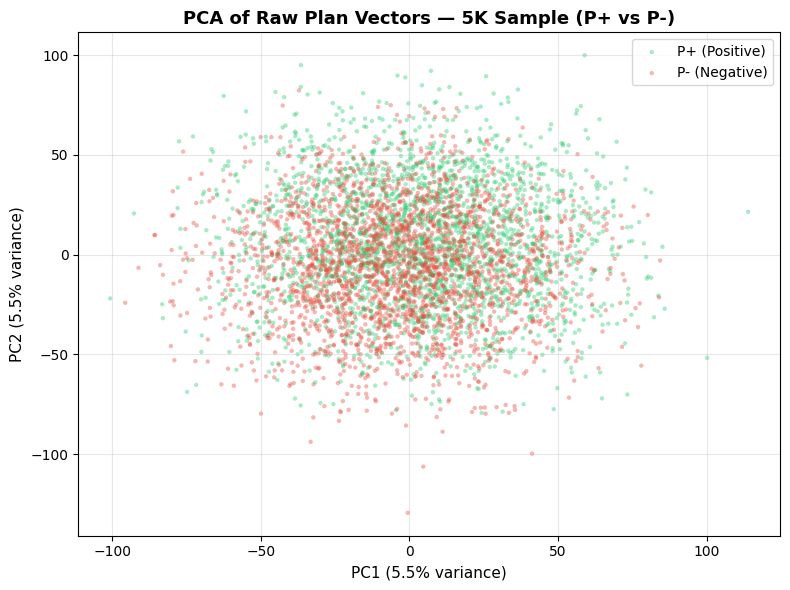
\includegraphics[width=0.78\textwidth]{figures/05_pca_raw.png}
    \caption{PCA visualization of the raw Gen-MOR 50K objective vectors. Points are colored by dominance label, where $P^{+}$ denotes nondominated plans and $P^{-}$ denotes dominated plans.}
    \label{fig:raw_dataset_pca}
\end{figure}

The PCA visualization in Fig.~\ref{fig:raw_dataset_pca} does not define dominance validity, but it helps illustrate the difficulty of the learning problem. Since the classes are not perfectly separated in the first two principal components, reconstruction and classification metrics must be interpreted together with dominance-specific validation.

\subsection{Class Distribution Results}
\label{subsec:class_distribution_results}

The final dataset is near-balanced, containing $25{,}209$ $P^{+}$ plans and $24{,}791$ $P^{-}$ plans. This near balance prevents the classifier from achieving high accuracy simply by favoring one majority class. The distribution is summarized in Table~\ref{tab:result_class_distribution}.

\begin{table}[H]
\centering
\caption{Class distribution used in the Gen-MOR 50K experiment.}
\label{tab:result_class_distribution}
\begin{tabular}{lccc}
\hline
\textbf{Class} & \textbf{Symbol} & \textbf{Label} & \textbf{Count} \\
\hline
Nondominated plans & $P^{+}$ & $1$ & $25{,}209$ \\
Dominated plans & $P^{-}$ & $0$ & $24{,}791$ \\
\hline
Total & -- & -- & $50{,}000$ \\
\hline
\end{tabular}
\end{table}

\begin{figure}[H]
    \centering
    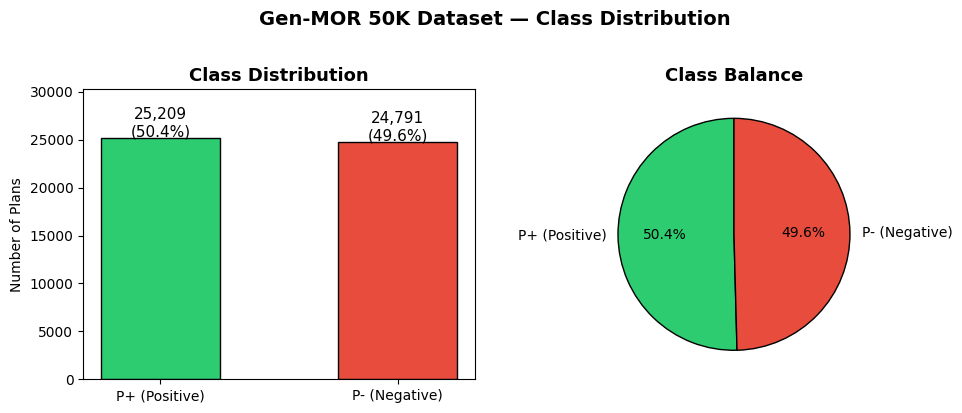
\includegraphics[width=0.80\textwidth]{figures/01_class_distribution.png}
    \caption{Class distribution of the Gen-MOR 50K dataset. The dataset is near-balanced, with $50.4\%$ $P^{+}$ plans and $49.6\%$ $P^{-}$ plans.}
    \label{fig:class_distribution}
\end{figure}

The near-balanced class distribution shown in Fig.~\ref{fig:class_distribution} makes classification metrics easier to interpret and provides comparable representation for both conditional generation targets in the CVAE.

\subsection{Autoencoder Training Results}
\label{subsec:ae_training_results}

The AE model is evaluated using total loss, reconstruction loss, and classification loss. The total loss follows Eq.~\eqref{eq:ae_total_loss}. During training, the reconstruction loss measures how well the decoder recovers objective vectors from the latent representation, while the classification loss measures how well the latent representation supports separation between $P^{+}$ and $P^{-}$.

\begin{figure}[H]
    \centering
    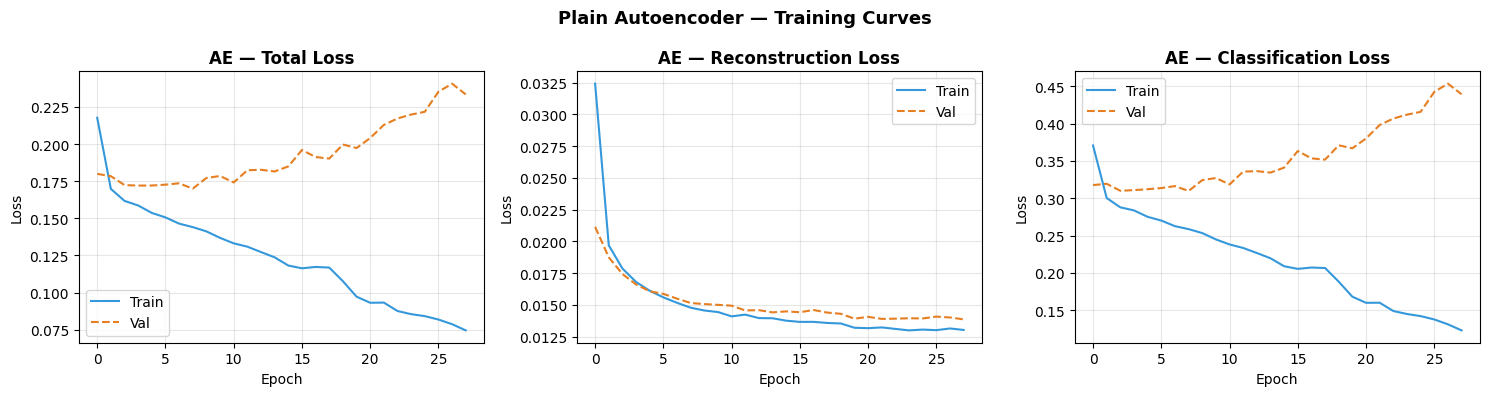
\includegraphics[width=1.0\textwidth]{figures/06_ae_loss_curves.png}
    \caption{AE training curves showing total loss, reconstruction loss, and classification loss over epochs.}
    \label{fig:ae_training_loss}
\end{figure}

The AE trained for $28$ epochs before early stopping. On the test set, it achieved a reconstruction MSE of $0.0150$, classification accuracy of $85.8\%$, and weighted F1 score of $0.8584$. These results show that the deterministic autoencoder learns a useful compressed representation for reconstructing MORNP-style objective vectors and predicting dominance labels.

\subsection{VAE Training Results}
\label{subsec:vae_training_results}

The VAE model is evaluated using total loss, reconstruction loss, KL divergence, and classification loss. The total loss follows Eq.~\eqref{eq:vae_total_loss}. Unlike the AE, the VAE must balance reconstruction quality with latent-space regularization. Therefore, the KL-divergence curve is an important part of the training analysis.

\begin{figure}[H]
    \centering
    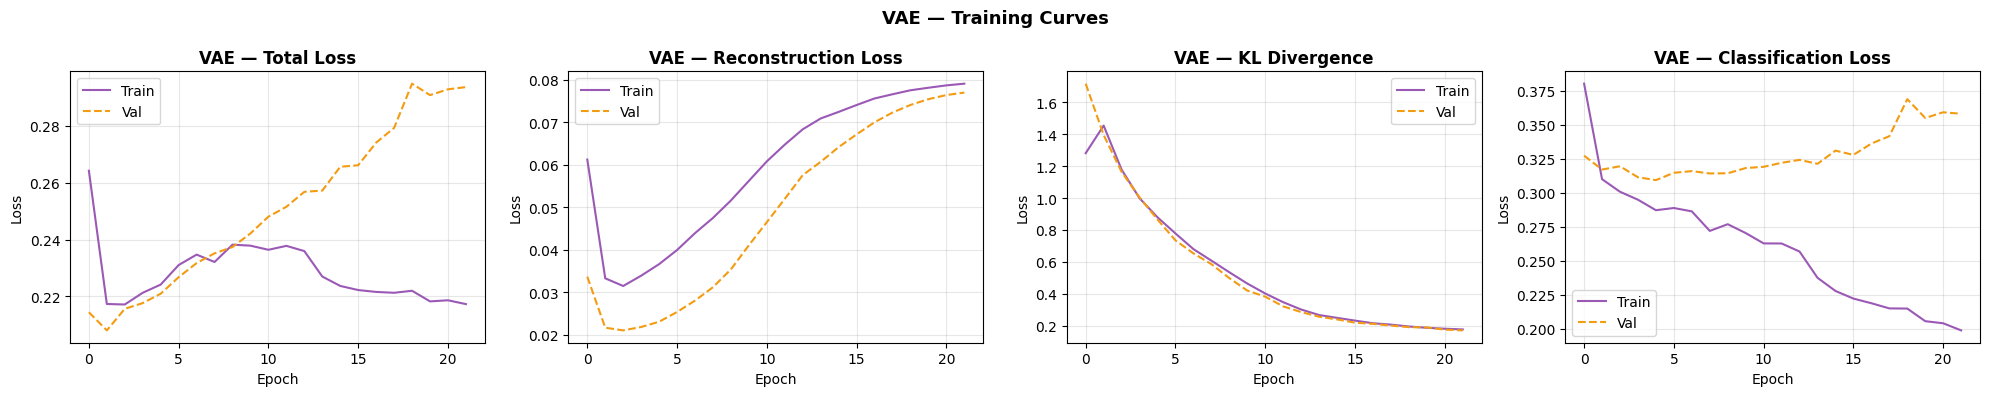
\includegraphics[width=1.0\textwidth]{figures/08_vae_loss_curves.png}
    \caption{VAE training curves showing total loss, reconstruction loss, KL divergence, and classification loss over epochs.}
    \label{fig:vae_training_loss}
\end{figure}

The VAE trained for $22$ epochs before early stopping. On the test set, it achieved a reconstruction MSE of $0.0215$, classification accuracy of $85.4\%$, and weighted F1 score of $0.8537$. Compared with the AE, the VAE has slightly higher reconstruction error, which is expected because the latent space is regularized for sampling. However, its classification performance remains close to that of the AE, indicating that the probabilistic latent representation still captures useful class-relevant structure.

\subsection{CVAE Training Results}
\label{subsec:cvae_training_results}

The CVAE model is evaluated using total loss, reconstruction loss, KL divergence, and classification loss. The total loss follows Eq.~\eqref{eq:cvae_total_loss}. The main difference between the CVAE and VAE is that the CVAE receives the dominance label as a conditioning input. This makes it possible to generate samples intended for a specific class, as shown in Eq.~\eqref{eq:cvae_positive_generation} and Eq.~\eqref{eq:cvae_negative_generation}.

\begin{figure}[H]
    \centering
    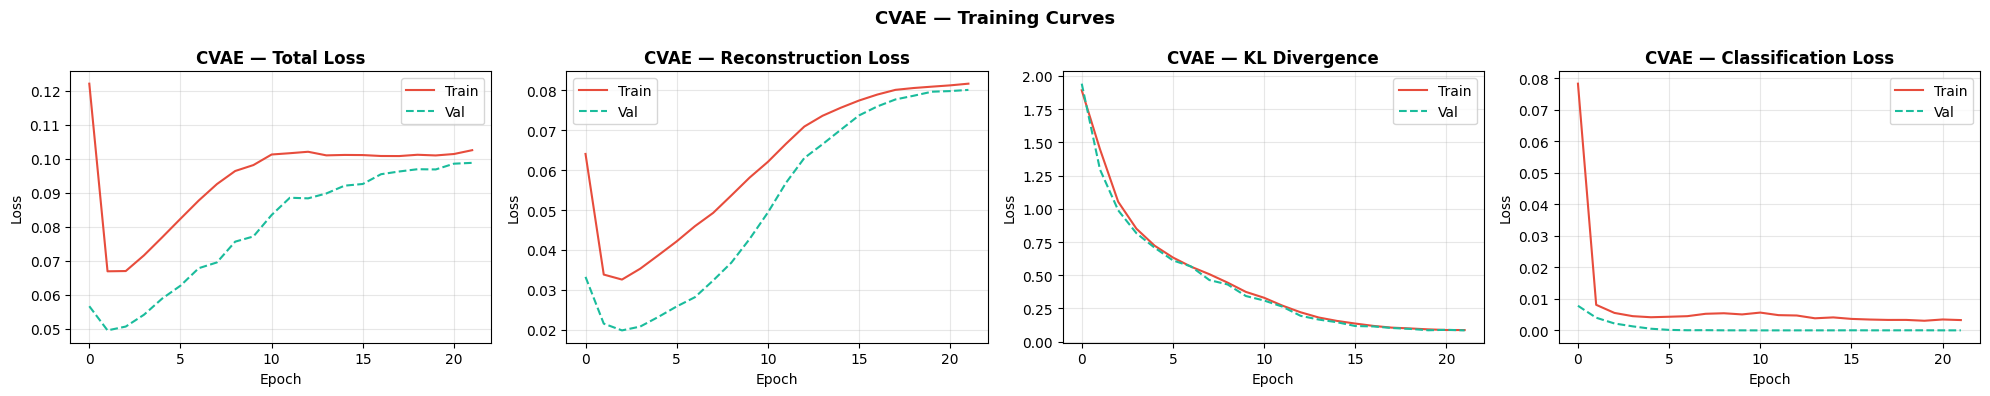
\includegraphics[width=1.0\textwidth]{figures/10_cvae_loss_curves.png}
    \caption{CVAE training curves showing total loss, reconstruction loss, KL divergence, and classification loss over epochs.}
    \label{fig:cvae_training_loss}
\end{figure}

The CVAE trained for $22$ epochs before early stopping. On the test set, it achieved a reconstruction MSE of $0.0213$, classification accuracy of $67.4\%$, and weighted F1 score of $0.6741$. The reconstruction error is close to the VAE result, but the classification score is lower. This suggests that while the CVAE can reconstruct objective vectors and enables class-conditioned generation, its learned latent representation is less effective for separating $P^{+}$ and $P^{-}$ in this experiment.

\subsection{Latent Space Analysis}
\label{subsec:latent_space_analysis}

Latent-space analysis is used to inspect whether the models learn representations that preserve class structure. For each trained model, latent representations are extracted and projected into two dimensions using PCA:
\begin{equation}
    \mathbf{v}_i
    =
    \operatorname{PCA}_2(\mathbf{z}_i),
    \qquad
    \mathbf{v}_i \in \mathbb{R}^{2}.
    \label{eq:latent_pca_projection}
\end{equation}

\begin{figure}[H]
    \centering
    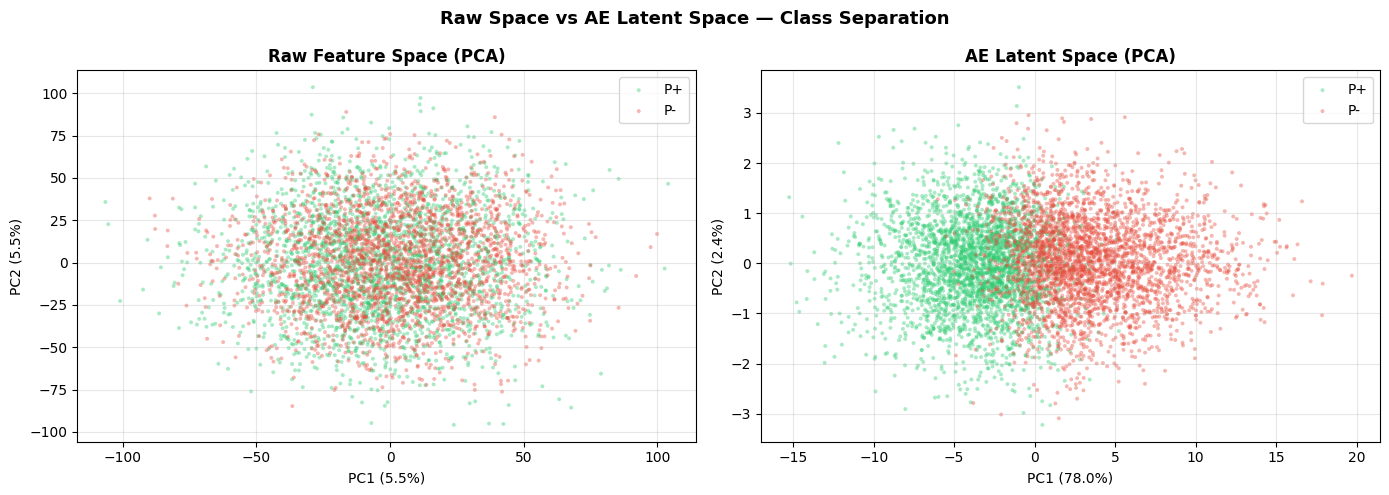
\includegraphics[width=0.90\textwidth]{figures/07_ae_latent_space.png}
    \caption{PCA visualization comparing the raw feature space and the AE latent space. Points are colored by $P^{+}$ and $P^{-}$ labels.}
    \label{fig:latent_space_pca}
\end{figure}

If the latent PCA plot shows stronger class organization than the raw PCA plot, this suggests that the model has learned a representation that captures dominance-relevant information. However, latent separation alone is not enough to prove dominance-preserving generation. Generated samples must still be checked using DVR.

\subsection{Reconstruction and Classification Comparison}
\label{subsec:reconstruction_classification_comparison}

The final reconstruction and classification results are compared across AE, VAE, and CVAE in Table~\ref{tab:model_performance_comparison}. These values are computed on the held-out test set of $7{,}500$ plans.

\begin{table}[H]
\centering
\caption{Reconstruction and classification comparison across Gen-MOR models on the 50K dataset.}
\label{tab:model_performance_comparison}
\begin{tabular}{|l|c|c|c|}
\hline
\textbf{Model} & \textbf{MSE} & \textbf{Accuracy} & \textbf{Weighted F1 Score} \\
\hline
AE & $0.0150$ & $85.8\%$ & $0.8584$ \\
VAE & $0.0215$ & $85.4\%$ & $0.8537$ \\
CVAE & $0.0213$ & $67.4\%$ & $0.6741$ \\
\hline
\end{tabular}
\end{table}

The AE achieves the lowest reconstruction error and the highest classification performance among the three models. The VAE performs slightly worse in reconstruction but remains close to the AE in classification, while also supporting latent-space generation. The CVAE provides class-conditioned generation, but its lower classification performance suggests that conditioning alone does not guarantee stronger class separation. More importantly, the best model under standard reconstruction and classification metrics is not necessarily the best model for dominance-preserving generation. Therefore, the next section evaluates generated samples using DVR.
%
\section{Dominance Validity Analysis}
\label{sec:dominance_validity_analysis}

This section evaluates whether the generative models produce samples that preserve the intended dominance structure. While Section~\ref{sec:experimental_results} evaluates reconstruction and classification, this section focuses on the central structural question of Gen-MOR: whether generated $P^{+}$ samples remain nondominated and generated $P^{-}$ samples remain dominated under the selected objective subset $S$. In the 50K experiment, DVR is computed using chunked vectorized verification with a reference pool of $10{,}000$ real plans and a generated-sample evaluation cap of $500$ samples per class.

\subsection{Generated $P^{+}$ Validity}
\label{subsec:generated_positive_validity}

Generated $P^{+}$ samples are expected to remain nondominated. For each generated positive sample $\tilde{p}^{+}_i$, the dominance verifier checks whether any plan in the verification pool $\mathcal{V}$ dominates it under the selected objective subset $S$. The positive dominance validity is computed using Eq.~\eqref{eq:positive_dvr}.

The results for generated $P^{+}$ samples are summarized in Table~\ref{tab:positive_dvr_results}.

\begin{table}[H]
\centering
\caption{Positive dominance validity for generated $P^{+}$ samples.}
\label{tab:positive_dvr_results}
\begin{tabular}{|l|c|c|c|}
\hline
\textbf{Model} & \textbf{Evaluated $P^{+}$ Samples} & \textbf{Valid $P^{+}$ Samples} & $\mathbf{DVR^{+}}$ \\
\hline
VAE & $327$ & $287$ & $87.8\%$ \\
CVAE & $500$ & $340$ & $68.0\%$ \\
\hline
\end{tabular}
\end{table}

A high $\operatorname{DVR}^{+}$ means that the model can generate samples that remain on the nondominated side of the dominance structure. In this experiment, the VAE achieves stronger positive dominance validity than the CVAE. The VAE generated $P^{+}$ set achieved $87.8\%$ positive DVR, while the CVAE achieved $68.0\%$. This suggests that VAE-generated positive samples more frequently remain nondominated under the selected MORNP objective subset.

\subsection{Generated $P^{-}$ Validity}
\label{subsec:generated_negative_validity}

Generated $P^{-}$ samples are expected to remain dominated. For each generated negative sample $\tilde{p}^{-}_i$, the verifier checks whether at least one plan in the verification pool $\mathcal{V}$ dominates it under $S$. The negative dominance validity is computed using Eq.~\eqref{eq:negative_dvr}.

The results for generated $P^{-}$ samples are summarized in Table~\ref{tab:negative_dvr_results}.

\begin{table}[H]
\centering
\caption{Negative dominance validity for generated $P^{-}$ samples.}
\label{tab:negative_dvr_results}
\begin{tabular}{|l|c|c|c|}
\hline
\textbf{Model} & \textbf{Evaluated $P^{-}$ Samples} & \textbf{Valid $P^{-}$ Samples} & $\mathbf{DVR^{-}}$ \\
\hline
VAE & $500$ & $227$ & $45.4\%$ \\
CVAE & $500$ & $206$ & $41.2\%$ \\
\hline
\end{tabular}
\end{table}

A high $\operatorname{DVR}^{-}$ means that the model generates samples that correctly remain dominated. In this experiment, negative dominance validity is noticeably lower than positive dominance validity for both models. The VAE achieves $45.4\%$ negative DVR, while the CVAE achieves $41.2\%$. This indicates that generating dominated samples is more difficult than generating nondominated samples in the current Gen-MOR setting.

\subsection{VAE and CVAE DVR Comparison}
\label{subsec:vae_cvae_dvr_comparison}

The VAE and CVAE provide different generation mechanisms. The VAE generates samples from an unconditional latent prior, while the CVAE generates samples conditioned on the target label. Because of this, the CVAE is expected to provide better class control. However, class conditioning does not automatically guarantee dominance validity.

Table~\ref{tab:dvr_comparison} compares the class-specific and overall DVR values. The overall DVR is computed from the evaluated generated samples in Tables~\ref{tab:positive_dvr_results} and~\ref{tab:negative_dvr_results}.

\begin{table}[H]
\centering
\caption{Dominance Validity Rate comparison for generated samples.}
\label{tab:dvr_comparison}
\begin{tabular}{|l|c|c|c|}
\hline
\textbf{Model} & $\mathbf{DVR^{+}}$ & $\mathbf{DVR^{-}}$ & \textbf{Overall DVR} \\
\hline
VAE & $87.8\%$ & $45.4\%$ & $62.2\%$ \\
CVAE & $68.0\%$ & $41.2\%$ & $54.6\%$ \\
\hline
\end{tabular}
\end{table}

\begin{figure}[H]
    \centering
    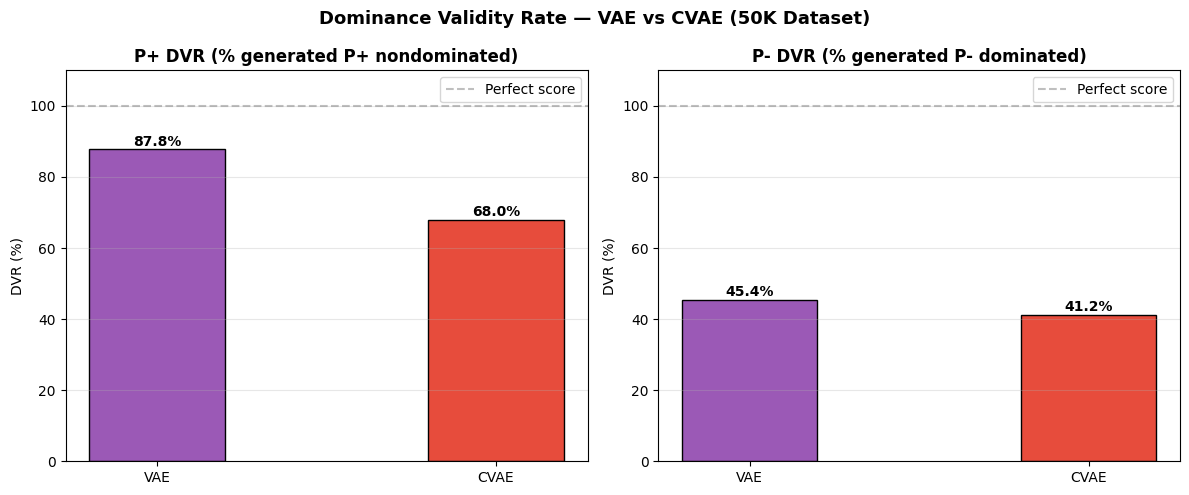
\includegraphics[width=0.90\textwidth]{figures/12_dvr_results.png}
    \caption{Dominance Validity Rate comparison between VAE and CVAE on the Gen-MOR 50K dataset. The left plot shows $P^{+}$ DVR, and the right plot shows $P^{-}$ DVR.}
    \label{fig:dvr_results}
\end{figure}

The comparison in Table~\ref{tab:dvr_comparison} and Fig.~\ref{fig:dvr_results} should be interpreted together with reconstruction and classification performance. Although the CVAE enables class-conditioned generation, it does not outperform the VAE on dominance validity in this experiment. The VAE achieves higher $\operatorname{DVR}^{+}$, higher $\operatorname{DVR}^{-}$, and higher overall DVR. This shows that class conditioning alone is not sufficient to guarantee dominance-preserving generation.

\subsection{Interpretation of DVR Variance}
\label{subsec:dvr_variance_interpretation}

DVR can vary across random seeds because generated samples depend on several stochastic factors. These include network initialization, mini-batch ordering, latent sampling, and the learned geometry of the latent space. Small differences during training may lead to different generated samples, and those generated samples may have different dominance behavior.

This variance is especially important for $P^{+}$ validity. A generated positive sample must avoid being dominated by any other plan in the verification pool. This is a stricter condition than merely resembling the distribution of positive training samples. Similarly, a generated negative sample must be dominated by at least one other plan, which requires the generated point to fall into a dominated region of the objective space.

The single-run DVR results in this section show that VAE performs better than CVAE on both positive and negative DVR. The multi-seed DVR variance is reported in Section~\ref{sec:multi_seed_robustness}. If DVR variance is high across seeds, then the model is not yet stable as a dominance-preserving generator.

\subsection{Dominance Validity vs. Reconstruction Quality}
\label{subsec:dominance_vs_reconstruction}

One of the central observations in Gen-MOR is that reconstruction quality and dominance validity measure different properties. Reconstruction MSE compares an input vector with its reconstructed output. DVR compares a generated vector against other plans using the formal dominance relation.

Therefore, a model can achieve low MSE and still generate invalid samples. This is visible in the current experiment. The CVAE has reconstruction MSE close to the VAE, but it has lower dominance validity. For example, if a generated $P^{+}$ sample is numerically close to the training distribution but is dominated by another plan, then it is invalid under DVR. Similarly, a generated $P^{-}$ sample may look realistic but fail to be dominated by any other plan. This shows that dominance-preserving generation requires more than ordinary distribution learning.

\subsection{Implications for Constraint-Aware Generation}
\label{subsec:constraint_aware_generation_implications}

The DVR results have direct implications for future model design. If VAE or CVAE models achieve reasonable reconstruction and classification performance but weaker DVR, then dominance validity should be incorporated more directly into the learning process. One possible direction is to add a dominance-aware penalty term to the loss function. Another direction is to use rejection sampling or post-generation filtering based on dominance verification.

The broader implication is that Gen-MOR should be treated as a constraint-aware generative modeling problem. The goal is not only to generate samples that look like the training data, but to generate samples that satisfy a relational constraint defined over objective vectors. DVR provides the measurement needed to expose this gap.
%
\section{Multi-Seed Robustness Analysis}
\label{sec:multi_seed_robustness}

This section evaluates the stability of the Gen-MOR models across multiple random seeds. Since neural generative models are stochastic, a single run may not provide a reliable picture of model performance. Multi-seed evaluation helps determine whether reconstruction, classification, and dominance validity are consistent across independent runs.

\subsection{Motivation for Multi-Seed Evaluation}
\label{subsec:motivation_multiseed}

The AE, VAE, and CVAE models can be affected by random initialization, mini-batch ordering, train-validation-test splitting, latent sampling, and dataset generation. For VAE and CVAE models, generation also depends on random samples drawn from the latent prior. These sources of variation can change both standard metrics and DVR.

For this reason, the experiment is repeated over the seed set $\mathcal{R}$ defined in Eq.~\eqref{eq:random_seed_set}. In the current experiment,
\begin{equation}
    \mathcal{R} = \{42, 123, 456, 789, 2024\}.
    \label{eq:actual_multiseed_set}
\end{equation}
For each seed, the same training, evaluation, generation, and dominance verification pipeline is executed. The final results are reported using the mean and standard deviation defined in Eq.~\eqref{eq:metric_mean} and Eq.~\eqref{eq:metric_std}.

\subsection{Reconstruction Stability}
\label{subsec:reconstruction_stability}

Reconstruction stability is evaluated by comparing MSE across seeds. A stable model should have both low average MSE and low standard deviation. Table~\ref{tab:mse_multiseed} reports the multi-seed reconstruction results.

\begin{table}[H]
\centering
\caption{Multi-seed reconstruction stability measured by MSE.}
\label{tab:mse_multiseed}
\begin{tabular}{|l|c|c|}
\hline
\textbf{Model} & \textbf{Mean MSE} & \textbf{Std. Dev.} \\
\hline
AE & $0.0277$ & $0.0061$ \\
VAE & $0.0579$ & $0.0185$ \\
CVAE & $0.0670$ & $0.0242$ \\
\hline
\end{tabular}
\end{table}

The AE has the lowest average reconstruction error and the smallest reconstruction variance. This indicates that the deterministic autoencoder is the most stable model for reconstructing objective-vector plans. The VAE and CVAE have higher mean MSE and larger standard deviation, which suggests that probabilistic latent regularization and conditional generation introduce additional variability across seeds.

\subsection{Classification Stability}
\label{subsec:classification_stability}

Classification stability is evaluated using accuracy and F1 score across seeds. Table~\ref{tab:classification_multiseed} summarizes the mean and standard deviation of these metrics.

\begin{table}[H]
\centering
\caption{Multi-seed classification stability.}
\label{tab:classification_multiseed}
\begin{tabular}{|l|c|c|c|c|}
\hline
\textbf{Model} & \textbf{Mean Accuracy} & \textbf{Accuracy Std.} & \textbf{Mean F1} & \textbf{F1 Std.} \\
\hline
AE & $83.2\%$ & $1.5\%$ & $0.8320$ & $0.0145$ \\
VAE & $82.8\%$ & $1.4\%$ & $0.8279$ & $0.0142$ \\
CVAE & $58.6\%$ & $4.2\%$ & $0.5681$ & $0.0422$ \\
\hline
\end{tabular}
\end{table}

The AE and VAE show similar and relatively stable classification performance across seeds. Their accuracy and F1 standard deviations are small compared with the CVAE. The CVAE has lower mean accuracy and F1 score, with larger variance. This indicates that, although the CVAE supports class-conditioned generation, its learned representation is less stable for separating $P^{+}$ and $P^{-}$ in the current experiment.

Stable classification results indicate that the models consistently learn a representation that separates $P^{+}$ and $P^{-}$. However, classification stability does not necessarily imply dominance-valid generation, which is evaluated separately.

\subsection{DVR Stability}
\label{subsec:dvr_stability}

DVR stability is the most important robustness measure for Gen-MOR because it evaluates whether dominance validity is consistent across runs. Table~\ref{tab:dvr_multiseed} reports the mean and standard deviation of $\operatorname{DVR}^{+}$ and $\operatorname{DVR}^{-}$.

\begin{table}[H]
\centering
\caption{Multi-seed dominance validity stability.}
\label{tab:dvr_multiseed}
\begin{tabular}{|l|c|c|c|c|}
\hline
\textbf{Model} &
\textbf{Mean $\mathbf{DVR^{+}}$} &
\textbf{Std.} &
\textbf{Mean $\mathbf{DVR^{-}}$} &
\textbf{Std.} \\
\hline
VAE & $57.7\%$ & $47.3\%$ & $49.6\%$ & $24.9\%$ \\
CVAE & $55.0\%$ & $31.8\%$ & $59.5\%$ & $29.8\%$ \\
\hline
\end{tabular}
\end{table}

The DVR results show that dominance-valid generation is much less stable than reconstruction and classification. The VAE has a slightly higher mean $P^{+}$ DVR than the CVAE, but its $P^{+}$ DVR standard deviation is very large. The CVAE has a higher mean $P^{-}$ DVR than the VAE, but it also shows substantial variance. This indicates that neither VAE nor CVAE consistently preserves dominance validity across seeds.

A model with high DVR but high standard deviation is not fully reliable, because its generated dominance validity depends strongly on the seed. A model with high DVR and low standard deviation is more desirable because it consistently generates structurally valid samples.

\begin{figure}[H]
    \centering
    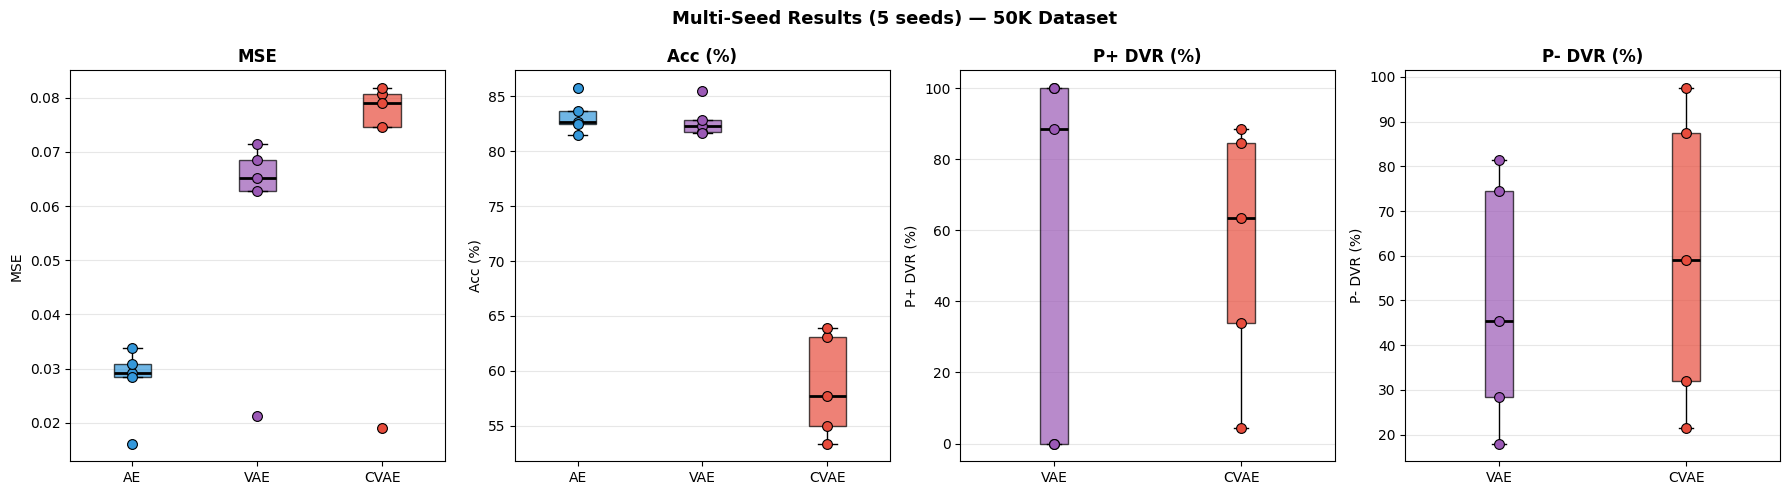
\includegraphics[width=1.0\textwidth]{figures/16_multiseed_boxplots.png}
    \caption{Multi-seed robustness results across reconstruction MSE, classification accuracy, $P^{+}$ DVR, and $P^{-}$ DVR.}
    \label{fig:multiseed_boxplots}
\end{figure}

Figure~\ref{fig:multiseed_boxplots} visually confirms the same trend as the tables. Reconstruction and classification results are comparatively more stable, especially for AE and VAE, while DVR has much larger variation across seeds.

\subsection{Robustness Summary}
\label{subsec:robustness_summary}

The multi-seed results should be interpreted across all metrics together. Reconstruction stability shows whether the model consistently learns the numerical objective-vector distribution. Classification stability shows whether the learned representation consistently separates $P^{+}$ and $P^{-}$. DVR stability shows whether generated samples consistently preserve the dominance relation.

The final robustness conclusion is summarized as follows:
\begin{compactitem}
    \item AE reconstruction stability: AE is the most stable reconstruction model, with the lowest mean MSE and lowest MSE standard deviation.
    \item VAE reconstruction and generation stability: VAE has stable classification performance close to AE, but its DVR is highly variable, especially for generated $P^{+}$ samples.
    \item CVAE class-controlled generation stability: CVAE enables class-conditioned generation, but it has weaker and less stable classification performance than AE and VAE.
    \item DVR stability across seeds: DVR is unstable for both VAE and CVAE, showing that dominance-preserving generation remains sensitive to random seed and latent sampling behavior.
\end{compactitem}

Since DVR variance remains high, the experiment supports the conclusion that dominance-preserving generation requires stronger constraint-aware learning mechanisms.
%
\section{Discussion}
\label{sec:discussion}

This section interprets the experimental findings and explains what they imply for generative modeling in MORNP-style multi-objective planning. The discussion focuses on the relationship between reconstruction, classification, conditional generation, and dominance validity.

\subsection{Main Findings}
\label{subsec:discussion_main_findings}

The main findings of the Gen-MOR 50K experiment can be summarized as follows. First, the AE and VAE models learn useful representations of MORNP-style objective vectors. The AE achieves the best reconstruction result, with a test MSE of $0.0150$, classification accuracy of $85.8\%$, and weighted F1 score of $0.8584$. The VAE achieves slightly higher reconstruction error, with MSE $0.0215$, but its classification performance remains close to the AE, with accuracy $85.4\%$ and weighted F1 score $0.8537$. This shows that probabilistic latent regularization reduces reconstruction sharpness slightly, but still preserves useful class-relevant information.

Second, the CVAE provides an important capability that the AE and ordinary VAE do not directly provide: class-conditioned generation. By conditioning on $y=1$ or $y=0$, the CVAE can explicitly generate samples intended to belong to $P^{+}$ or $P^{-}$. However, the current experiment shows that this class-control mechanism does not automatically improve classification or dominance validity. The CVAE achieves test MSE $0.0213$, which is close to the VAE, but its classification accuracy drops to $67.4\%$ and its weighted F1 score drops to $0.6741$.

Third, the DVR results show that dominance-valid generation is more difficult than reconstruction or classification. In the single-run experiment, the VAE achieves $87.8\%$ $P^{+}$ DVR and $45.4\%$ $P^{-}$ DVR, while the CVAE achieves $68.0\%$ $P^{+}$ DVR and $41.2\%$ $P^{-}$ DVR. Therefore, VAE performs better than CVAE on both positive and negative dominance validity in the current run. However, the multi-seed results show that DVR varies substantially across seeds, which means that dominance-valid generation is still not stable.

Finally, the comparison between standard metrics and DVR shows that reconstruction performance does not automatically guarantee dominance validity. The CVAE has reconstruction error close to the VAE, but it performs worse in classification and DVR. This distinction is central to the contribution of Gen-MOR: generated samples must be evaluated not only by numerical similarity, but also by whether they satisfy the formal dominance relation.

\subsection{Why AE and VAE Perform Strongly on Reconstruction}
\label{subsec:why_ae_vae_reconstruct_well}

The AE and VAE perform strongly on reconstruction because the input data consists of fixed-length numerical vectors. Compared with images, graphs, or sequences, objective vectors have a simpler structure and a fixed dimensionality. The models do not need to learn variable-length dependencies or discrete syntax. Instead, they learn correlations among objective dimensions and compress these correlations into a latent representation.

The AE is particularly well suited for reconstruction because it directly optimizes a deterministic encoding and decoding path. This explains why it obtains the lowest MSE among the three models. The VAE has slightly higher reconstruction error because it also regularizes the latent distribution using the KL-divergence term. This regularization can reduce reconstruction accuracy, but it makes the latent space more suitable for sampling and generation.

\subsection{Why CVAE Is Useful but Less Stable}
\label{subsec:why_cvae_useful_less_stable}

The CVAE is useful because it supports class-controlled generation. In Gen-MOR, this means that the model can be asked to generate a sample intended for $P^{+}$ or $P^{-}$. This is a major advantage over unconditional generation because the experiment requires separate evaluation of generated nondominated and dominated samples.

However, the current experiment shows that conditioning alone is not enough to produce stronger dominance-aware generation. Although the dataset is near-balanced, with $25{,}209$ $P^{+}$ plans and $24{,}791$ $P^{-}$ plans, the CVAE still has weaker classification performance than AE and VAE. This suggests that the difficulty is not mainly caused by class imbalance. Instead, the challenge is likely caused by the conditional latent modeling problem and by the relational nature of dominance. The decoder must learn how the label changes the structure of the generated objective vector, but validity still depends on comparison against other plans.

\subsection{Why Dominance-Aware Generation Is Difficult}
\label{subsec:why_dominance_generation_difficult}

Dominance-aware generation is difficult because dominance is relational rather than pointwise. A model can generate a vector that looks realistic in isolation, but whether that vector belongs to $P^{+}$ or $P^{-}$ depends on how it compares with other plans under the selected objective subset $S$.

This makes Gen-MOR different from ordinary binary generation. In a standard classification setting, a generated sample may be judged by whether it resembles one class or another. In Gen-MOR, the generated sample must satisfy a formal comparison rule. A valid $P^{+}$ sample must not be dominated by any relevant plan, while a valid $P^{-}$ sample must be dominated by at least one relevant plan. These conditions are harder to learn because they depend on the geometry of the entire plan set.

The current DVR results support this point. Both VAE and CVAE achieve lower $P^{-}$ DVR than $P^{+}$ DVR in the single-run experiment. This means that generating dominated samples is especially difficult. A generated $P^{-}$ sample must fall into a region where at least one reference plan dominates it, which is a stricter relational requirement than simply producing a plausible-looking objective vector.

\subsection{Research Significance}
\label{subsec:research_significance}

The significance of Gen-MOR is that it treats generative modeling as a structure-preserving task for multi-objective reasoning. The goal is not only to generate realistic samples, but to generate samples that remain logically consistent with dominance rules. This moves the evaluation beyond ordinary reconstruction and classification.

This is important for planning and decision-support systems because synthetic data may be used to stress-test algorithms, augment training sets, or explore new regions of the objective space. If generated samples violate the dominance structure, they may mislead downstream solvers or evaluators. Therefore, dominance validity must be measured explicitly. DVR provides this structural evaluation and exposes errors that MSE, accuracy, and F1 score cannot detect.

\subsection{Comparison with Pareto-Guided Generative Models}
\label{subsec:comparison_pareto_guided_models}

Existing Pareto-guided generative models often focus on approximating or improving the Pareto front. For example, latent-space optimization, ParetoFlow, and Pareto-guided diffusion approaches are designed to generate samples that move toward Pareto-optimal regions or improve multi-objective trade-offs. These methods are valuable for optimization-focused generation.

Gen-MOR is complementary to those approaches. Instead of focusing only on Pareto-front improvement, it studies whether generated samples preserve a dominance-based class structure. In this setting, both $P^{+}$ and $P^{-}$ are important. The model must generate nondominated plans and dominated plans, and each generated sample must be checked using the formal dominance relation. This makes DVR a necessary evaluation metric for Gen-MOR.

The current results show that ordinary AE/VAE/CVAE-style generative modeling can learn useful numerical representations, but does not yet guarantee stable dominance-preserving generation. This suggests that future work should move toward explicitly dominance-constrained objectives, post-generation verification, or more advanced Pareto-guided generative models adapted to the MORNP setting.
%
\section{Limitations}
\label{sec:limitations}

Although the Gen-MOR experiment provides a useful framework for dominance-preserving generative modeling, several limitations remain. These limitations help clarify what the current experiment demonstrates and what should be improved in future work.

The dataset is generated from a synthetic MORNP-style construction process rather than from a real deployed planning system. This is useful for controlled experimentation because the dominance labels can be verified using the formal dominance relation. However, real-world planning data may contain additional structure, noise, constraints, and domain-specific dependencies that are not fully captured by the synthetic generator. Although the current 50K-plan dataset is substantially larger than the preliminary 1K dataset, it is still a controlled synthetic benchmark rather than a real-world deployment dataset.

The objectives in the current dataset are represented as generic numerical dimensions such as \texttt{obj\_1}, \texttt{obj\_2}, and so on. This makes the experiment general, but it also limits semantic interpretation. In a real planning domain, objectives may correspond to specific quantities such as cost, time, risk, energy, or safety. Future versions should connect the objective dimensions to a concrete planning environment so that generated plans can be interpreted not only structurally, but also semantically.

The current experiment focuses on AE, VAE, and CVAE models. These models are appropriate for a first Gen-MOR study because they provide a clear progression from reconstruction to probabilistic generation and class-conditioned generation. However, the experiment does not yet include more advanced generative architectures such as energy-based models, normalizing flows, diffusion models, or hybrid constraint-guided generators.

The current models are evaluated using DVR, but dominance validity is not directly optimized during training. The loss functions include reconstruction, classification, and KL-divergence terms, but they do not include a differentiable dominance penalty. As a result, a model may learn to reconstruct and classify objective vectors reasonably well without learning to generate dominance-valid samples consistently. This limitation is visible in the gap between standard reconstruction/classification metrics and DVR results.

Generated samples may vary significantly across random seeds. Even if a model achieves good average reconstruction and classification performance, its DVR may still fluctuate across runs. The multi-seed results show that DVR has much higher variance than reconstruction and classification metrics, especially for VAE and CVAE generation. This indicates that dominance-preserving generation is not yet stable. This limitation is addressed partially through multi-seed evaluation, but future models should aim to reduce this instability.

Dominance verification can become computationally expensive because it requires comparing generated samples against a verification pool under the selected objective subset. In the current 50K experiment, DVR computation is made practical using chunked vectorized verification with a reference pool of $10{,}000$ real plans and a generated-sample evaluation cap of $500$ samples. As the number of generated samples, reference plans, or objectives increases, DVR computation may become a bottleneck. Efficient dominance-checking strategies may be needed for larger-scale experiments.

The current experiment evaluates generated plans using formal dominance checks, but it does not yet test whether the generated plans improve a downstream planner, solver, or decision-support workflow. Therefore, the results demonstrate feasibility for dominance-preserving generation, but they do not yet prove real-world planning utility.
%
\section{Future Work}
\label{sec:future_work}

The Gen-MOR framework opens several directions for future research. The most important direction is to move from post-hoc dominance verification toward models that directly optimize dominance validity during training. The current experiment shows that AE, VAE, and CVAE models can learn useful numerical representations of MORNP-style objective vectors, but the DVR results also show that dominance-preserving generation remains unstable. Therefore, future work should focus on making dominance validity part of the learning and sampling process rather than only a post-generation evaluation step.

A natural next step is to add a dominance-aware loss term to the training objective. Instead of evaluating dominance validity only after generation, the model could be penalized during training when generated samples violate the intended dominance condition. Such a term could be written generally as
\begin{equation}
    \mathcal{L}_{Gen\text{-}MOR}
    =
    \mathcal{L}_{model}
    +
    \lambda_{dom}\mathcal{L}_{dom},
    \label{eq:future_dominance_loss}
\end{equation}
where $\mathcal{L}_{model}$ is the original AE, VAE, or CVAE loss, $\mathcal{L}_{dom}$ is a dominance-violation penalty, and $\lambda_{dom}$ controls its strength. This direction is especially important for VAE and CVAE generation, because these models produce new samples whose validity must be checked against the Pareto dominance relation.

The final experiment uses a near-balanced 50K dataset with $25{,}209$ $P^{+}$ plans and $24{,}791$ $P^{-}$ plans. Future work can improve the dataset generation process further by controlling not only class counts, but also the diversity and difficulty of the samples in each class. For example, dominated plans can be generated with different degrees of domination, and nondominated plans can be generated from different regions of the Pareto front. This would allow the experiment to test whether generative models can learn easy, moderate, and difficult dominance cases separately.

The CVAE provides class-controlled generation, but the current experiment shows that class conditioning alone does not guarantee better dominance validity. Future work can improve the conditioning mechanism using learned class embeddings, stronger label-conditioning layers, contrastive latent separation, or separate latent priors for $P^{+}$ and $P^{-}$. These methods may help the model generate more reliable class-specific samples and reduce the gap between intended class labels and actual dominance validity.

Energy-based models provide a promising direction because they can assign low energy to valid samples and high energy to invalid samples. In the Gen-MOR setting, an EBM could be trained to assign lower energy to dominance-valid plans and higher energy to dominance-invalid plans. This would allow dominance validity to become part of the sampling process rather than only a post-generation check.

Future work can also extend Gen-MOR to diffusion models or normalizing flows. Diffusion models may provide more stable sample generation, while flow-based models provide exact likelihoods and invertible transformations. A Pareto-guided or dominance-guided diffusion model could gradually denoise samples toward regions that satisfy the desired $P^{+}$ or $P^{-}$ conditions. Similarly, a flow-based Gen-MOR model could learn a structured mapping between latent variables and dominance-valid objective vectors.

Although the current experiment uses $50{,}000$ plans, future experiments can vary the dataset size, number of objectives, number of selected objectives, number of generated samples, reference pool size, and number of random seeds. This would help determine how Gen-MOR scales with objective dimensionality and plan-set complexity. Larger experiments could also test whether DVR becomes more stable when the models are trained on more diverse examples.

Another direction is to integrate generated plans with MORNP solver workflows. Generated samples could be used to augment plan sets, create stress-test instances, or evaluate how solvers behave under larger and more diverse dominance structures. This would connect Gen-MOR more directly to the original MORNP motivation and could show whether generative modeling improves downstream multi-objective reasoning tasks.
%
\section{Conclusion}
\label{sec:conclusion}

This project introduced Gen-MOR, a generative modeling framework for MORNP-style multi-objective plan vectors. Each plan is represented as an objective vector and assigned a dominance-based label: $P^{+}$ for nondominated plans and $P^{-}$ for dominated plans. The central goal is to learn models that can reconstruct, classify, and generate plan vectors while preserving the dominance structure defined by Pareto dominance.

The experiment evaluates three neural architectures: AE, VAE, and CVAE. The AE provides a deterministic representation-learning baseline, the VAE introduces probabilistic latent generation, and the CVAE enables class-conditioned generation for $P^{+}$ and $P^{-}$ samples. These models are evaluated using reconstruction MSE, classification accuracy, precision, recall, F1 score, and KL divergence where applicable.

The main contribution of Gen-MOR is the use of Dominance Validity Rate as a structural evaluation metric. DVR directly measures whether generated $P^{+}$ samples remain nondominated and whether generated $P^{-}$ samples remain dominated under the selected objective subset. This is important because standard metrics alone cannot determine whether a generated sample is valid under the MORNP dominance structure.

The Gen-MOR 50K experiment shows that AE and VAE learn useful representations of MORNP-style objective vectors. The AE achieves the strongest reconstruction and classification performance, with MSE $0.0150$, accuracy $85.8\%$, and weighted F1 score $0.8584$. The VAE achieves slightly higher reconstruction error, with MSE $0.0215$, but maintains similar classification performance with accuracy $85.4\%$ and weighted F1 score $0.8537$. The CVAE achieves reconstruction MSE $0.0213$, but its classification performance is lower, with accuracy $67.4\%$ and weighted F1 score $0.6741$.

The dominance validity analysis shows that VAE performs better than CVAE in the single-run DVR evaluation. The VAE achieves $87.8\%$ $P^{+}$ DVR and $45.4\%$ $P^{-}$ DVR, while the CVAE achieves $68.0\%$ $P^{+}$ DVR and $41.2\%$ $P^{-}$ DVR. These results show that class-conditioned generation alone does not guarantee dominance-valid generation. The multi-seed analysis further shows that DVR has much higher variance than reconstruction and classification metrics, indicating that dominance-preserving generation remains unstable across random seeds.

Overall, the project supports the feasibility of using generative models for multi-objective reasoning data, but it also shows that dominance-preserving generation is more difficult than ordinary reconstruction or classification. Future work should therefore incorporate dominance constraints directly into the training process and explore more advanced generative architectures such as energy-based models, diffusion models, and flow-based models.
%
\bibliographystyle{splncs04}
\vspace{-10pt}
\bibliography{references}
\end{document}
